

\newpage



%----------------------------------------------------------------------------------------


%\section[Static Correlations][Corrélations Statiques]{Static correlations of urban form and network shape}{Corrélations Statiques entre Forme Urbaine et Forme de Réseau}
\section{Urban form and Network Topology}{Corrélations entre forme des territoires et forme des réseaux}




\label{sec:staticcorrelations}


%----------------------------------------------------------------------------------------



Au travers des processus de relocalisation, parfois induits par les réseaux, on peut s'attendre à ce que ces derniers influencent la distribution des populations dans l'espace. Réciproquement, les caractéristiques du réseau peuvent être influencées par celle-ci. Nous proposons ici d'étudier ces liens potentiels au travers de caractérisations issues d'indicateurs synthétiques pour ces deux sous-systèmes, et des corrélations entre ces indicateurs.

%les agrégats urbains se qualifient au dessus d'une certaine échelle par une forme urbaine, de même que les réseaux de transport présentent des propriétés topologiques synthétiques.\comment[FL]{le fait de quantifier ne signifie pas que ces proprietes existent}[(JR) pas d'accord, a partir du moment où on a un modèle on a necessairement une ontologie sous-jacente - je sais pas ce que tu veux dire exactement par existe ?][(FL) tu dis ``presentant des proprietes''. soit c'est juste un calcul d'indicateurs, pas forcement une propriete, soit il y a des proprietes ``observables'' (reseau en etoile, reseau maille, etc.) et effectivement les indicateurs peuvent les montrer. par ex. que dirais tu si le reseau reseemble à | X $\Gamma$ - |]

%\bpar{
%Spatio-temporal processes implying diffusion or propagation phenomena generally have a specific structure of correlation. In particular, as derived in section~\ref{sec:spatiotempcorrs}, a static computation of correlation between different instances of a system may under certain conditions provide information on dynamical correlations implied.
%}{
%Les processus spatio-temporels impliquant une diffusion ou une propagation\footnote{Ce qui est a priori le cas de la forme urbaine comme suggéré par~\ref{sec:densitygeneration} qui reproduit des formes urbaines à partir de ces processus.} peuvent être compris par l'intermédiaire de leur structure de covariance dans le temps et l'espace.
%}
% Dans certains cas, on peut espérer que l'étude d'une correlation statique entre différentes instances d'un système peuvent sous certaines conditions informer sur les correlations dynamiques sous-jacentes, ce que nous ferons de manière empirique ici.




\bpar{
At the macroscopic scale of system of cities, the spatial nature of the urban system is reasonably captured by cities position, associated with aggregated city variable to represent entirely the system (see e.g. ontologies of Simpop models~\cite{pumain2012multi} or its successor Marius~\cite{cottineau2014evolution}). At the mesoscopic scale at which we aim to capture morphological manifestations of interactions between transportation networks and territories, structure of the territorial system can be specified by more refined indicators for the morphological aspect.
}{
A l'échelle du système de villes, le caractère spatial du système urbain peut être synthétisé par les positions des villes, associées aux variables agrégées au niveau de la ville. Nous nous placerons ici à l'échelle mesoscopique, à laquelle la distribution spatiale fine des activités est nécessaire pour comprendre la structure spatiale du système territorial. Nous parlerons ainsi de caractéristiques morphologiques pour la densité de population et le réseau routier.
}


\bpar{}{
Le choix de limites ``pertinentes'' pour le territoire ou la ville est un problème relativement ouvert qui dépendra souvent de la question à laquelle on cherche à répondre \cite{paez2005spatial}. Ainsi, \cite{guerois2002commune} montrent que les entités obtenues sont différentes si on considère une entrée par la continuité du bâti (morphologique), par les fonctions urbaines (zones d'emploi par exemple) ou par les limites administratives. Nous choisissons ici l'échelle mesoscopique d'un centre métropolitain, de l'ordre de la centaine de kilomètres, d'une part pour la cohérence du champ spatial calculé, et d'autre part parce que des échelles plus grandes deviennent moins pertinentes pour la notion de forme urbaine, tandis que des échelles plus petites induisent une trop grande variabilité.
}

% \footnote{Par example, tenter de définir un territoire \emph{Parisien} présenterait plusieurs facettes. Du point de vue du territoire subjectif, les Parisiens intra-muros considèrent une barrière stricte au Boulevard Périphérique, tandis que des banlieues plus ou moins proches seront vues comme parisiennes depuis la province. Le territoire fonctionnel du Métropolitain s'étend légèrement plus loin que la limite administrative de Paris, mais couvre quasiment toute l'Ile-de-France lorsqu'on y ajoute RER et Transilien. Les périmètres de gouvernance sont en train d'évoluer avec le projet de gouvernance métropolitaine (voir~\ref{sec:casestudies}). Des perceptions complémentaires du territoires peuvent ainsi être multipliées.}


\bpar{
We study systematically morphological indicators for constant size areas covering a given geographical area. The choice of fixed size areas can be questioned regarding definition of a territorial system, that can be otherwise understood as a consistent spatial entity at a given scale and along certain criteria : \emph{Human territories} as defined by Raffestin (op. cit.) or more generally functionally autonomous spaces\footnote{for example, a tentative of definition of a \textit{Parisian} territory would present many facets. From the subjective territory point of view, intra-muros Parisians consider a strict boundary at \textit{Boulevard Periph{\'e}rique}, whereas close and even further suburbs will be seen as Parisians from the Province. The functional territory of \textit{Metropolitain} extends slightly further than the administrative boundary. Governance perimeters are currently mutating with the Metropolitan governance project. Complementary perceptions of the territory can thus be multiplied.}. Here we choose the mesoscopic scale of a metropolitan center ($\simeq$ 50km) for comparability purposes and because greater scale are no more relevant regarding urban form, whereas smaller scales must contain too much noise. 
}{
A cette échelle, on peut supposer les caractéristiques du territoire, pour la population et le réseau, définies localement et variant de manière relativement continue dans l'espace. Ainsi, la construction de champs d'indicateurs morphologiques permettra de reconstruire de manière endogène des ensembles territoriaux par la structure spatiale émergente des indicateurs aux échelles plus petites. Par exemple, les villes devraient se distinguer au sein des espaces non urbains. L'enjeu de cette section est ainsi d'étudier les propriétés de ces indicateurs et de leurs interactions, et donc indirectement les interactions entre territoire et réseau.
}




%%%%%%%%%%%%%%%%%%
\subsection{Morphological Measures}{Mesures morphologiques}

\subsubsection{Urban Morphology}{Morphologie Urbaine}


Les manières de quantifier et qualifier la \emph{forme urbaine} à l'échelle considérée, et par extension à toute distribution de population dans l'espace ce qu'on peut appeler \emph{forme territoriale}, sont nombreuses.

\bpar{
\cite{guerois2008built} studies the form of European cities using a simple measure of density slopes from the center to the periphery. We need however quantities having a certain level of robustness and invariance. For example, two polycentric cities should be classified as morphologically close whereas a direct comparison of distributions (with the Earth Mover Distance for example) could give a very high distance between configurations depending on center positions.
}{
Nous avons cependant besoin de mesures ayant un certain niveau d'invariance pour extraire des formes typiques. Par exemple, deux villes monocentriques, c'est à dire concentrées autour d'un point donné, devraient être mesurées comme morphologiquement proches par un indicateur de monocentrisme tandis qu'une comparaison directe des distributions de population pourra donner une distance très élevée\footnote{On peut comparer des distributions spatiales par une distance euclidienne entre les matrices correspondantes, ou par des distances plus élaborées comme la distance de Monge qui résout un problème de transport minimal et donne la quantité de déplacements nécessaires pour passer d'une distribution à l'autre.} entre les configurations selon la position des centres.
}



\bpar{
We choose to refer to the literature in Urban Morphology which proposes an extensive set of indicators to describe urban form~\cite{tsai2005quantifying}. The number of dimensions can be reduced to obtain a robust description with a few number of independent indicators~\cite{Schwarz201029}.
}{
Nous choisissons pour notre étude de nous référer à la littérature en morphologie urbaine qui propose des jeux d'indicateurs variés pour décrire la forme urbaine~\cite{tsai2005quantifying}. \cite{le2009quantifier} rappelle la nécessité d'une mesure multi-dimensionnelle de la forme urbaine. Il est possible d'obtenir une description robuste avec un petit nombre d'indicateurs indépendants par une réduction de la dimension~\cite{Schwarz201029}.
}


\bpar{
The use of fractal indexes is a possibility suggested by~\cite{2016arXiv160808839C}.
}{
D'autres solution existent pour quantifier la morphologie urbaine\footnote{Dans l'urbanisme opérationnel, la morphologie urbaine est définie comme ``les caractéristiques de la forme matérielle des villes et des tissus''~\cite{paquot2010abc}. Nous utilisons ce terme ici pour les tissus à une échelle mesoscopique, vu par la distribution spatiale des populations.}. \cite{guerois2008built} étudient la forme des villes Européennes par l'utilisation d'une mesure simple des gradients de densité du centre vers la périphérie. Il est aussi possible d'utiliser des indices issus de l'analyse fractale, comme par exemple appliquée systématiquement par~\cite{2016arXiv160808839C} pour classifier les formes urbaines. Le lien entre morphologie urbaine et topologie du graphe de relations sous-jacent a été suggéré dans une approche théorique par~\cite{badariotti2007conception}. D'autre indices plus originaux peuvent être proposés, comme par~\cite{lee2017morphology} qui utilise les variations de trajectoire d'itinéraires traversant une ville pour établir une classification et montrer que celle-ci est fortement corrélée aux variables socio-économiques.
}



\bpar{
 Note that here we consider indicators on population density only, and that more elaborated considerations on Urban Form include for example the distribution of economic opportunities and the combination of these two fields through accessibility measures. For the choice of indicators, we follow the analysis done in~\cite{le2015forme} in which a morphological typology of large european cities is obtained.
}{
Il faut noter que nous ne considérons ici des indicateurs sur la distribution spatiale de la densité de population uniquement, et que des considérations plus élaborées sur la forme urbaine peuvent inclure par exemple la distribution des opportunités économiques et la combinaison de ces deux champs par des mesures d'accessibilité. Pour le choix des indicateurs, nous suivons l'analyse faite par~\cite{le2015forme} où une typologie morphologique des grandes villes européennes est obtenue. La cohérence de celle-ci suggère la capacité du jeu d'indicateurs utilisé à capturer la forme urbaine à cette échelle. Nous nous trouvons à une échelle comparable et devons capturer des aspects divers comme la hiérarchie, la concentration, le degré d'acentrisme de la distribution de population, d'où l'utilisation d'indicateurs similaires.
}


\subsubsection{Indicators}{Indicateurs}

\bpar{
We give now the formal definition of morphological indicators. We consider gridded population data $(P_i)_{1\leq i \leq N^2}$, write $M=N^2$ the number of cells, $d_{ij}$ the distance between cells $i,j$, and $P=\sum_{i=1}^{M} P_i$ total population. We measure Urban Form using:

\begin{enumerate}
\item Rank-size slope $\gamma$, expressing the degree of hierarchy in the distribution, computed by fitting with Ordinary Least Squares a power law distribution by $\ln \left( P_{\tilde{i}}/P_0\right) \sim k + \gamma\cdot \ln \left(\tilde{i}/i_0\right)$ where $\tilde{i}$ are the indexes of the distribution sorted in decreasing order. It is always negative, and values close to zero mean a flat distribution.
\item Entropy of the distribution, that expresses how uniform the distribution is:
\begin{equation}
\mathcal{E} = \sum_{i=1}^{M}\frac{P_i}{P}\cdot \ln{\frac{P_i}{P}}
\end{equation}
$\mathcal{E}=0$ means that all the population is in one cell whereas $\mathcal{E}=0$ means that the population is uniformly distributed.
\item Spatial-autocorrelation given by Moran index, with simple spatial weights given by $w_{ij} = 1/d_{ij}$
\[
I = \frac{\sum_{i\neq j} w_{ij} \left(P_i - \bar{P}\right)\cdot\left(P_j - \bar{P}\right)}{\sum_{i\neq j} w_{ij} \sum_{i}{\left( P_i - \bar{P}\right)}^2}
\]
Positive values will imply aggregation spots (``density centers''), negative values strong local variations whereas $I=0$ corresponds to totally random population values.
\item Mean distance between individuals, which captures population concentration
\[
\bar{d} = \frac{1}{d_M}\cdot \sum_{i<j} \frac{P_i P_j}{P^2} \cdot d_{ij}
\]
where $d_M$ is a normalisation constant taken as the diagonal of the world in our case.
\end{enumerate}
}{
Nous donnons à présent une définition formelle des indicateurs morphologiques utilisés ici. Nous considérons des données de population en grille $(P_i)_{1\leq i \leq N^2}$, écrivons $M=N^2$ le nombre de cellules, $d_{ij}$ la distance euclidienne entre les cellules $i$ et $j$, $P=\sum_{i=1}^{M} P_i$ la population totale, et $\bar{P}=\frac{1}{M}\cdot\sum_{i=1}^{M} P_i$ la population moyenne. La forme urbaine est mesurée par : 

\begin{enumerate}
\item Pente de la loi rang-taille $\gamma$, qui exprime le degré de hiérarchie de la distribution, calculé en ajustant une loi de puissance par Moindres Carrés Ordinaires par $\ln \left( P_{\tilde{i}}/P_0\right) \sim k + \gamma\cdot \ln \left(\tilde{i}/i_0\right)$ où $\tilde{i}$ sont les indices de la distribution triée de manière décroissante (la constante $k$ de l'ajustement ne joue pas de rôle dans la hiérarchie). Elle est toujours négative ou nulle, et des valeurs proches de zéro signifient une distribution complètement homogène. %Son utilisation sur une grille est amenée de manière originale par~\cite{le2015forme}.
\item Entropie de la distribution~\cite{le2015forme}, qui exprime l'uniformité de la distribution, ce qui est une façon de capturer un niveau de concentration :
\begin{equation}
\mathcal{E} = \sum_{P_i\neq 0}\frac{P_i}{P}\cdot \ln{\frac{P_i}{P}}
\end{equation}
$\mathcal{E}=0$ signifie que toute la population est dans une cellule tandis que $\mathcal{E}=0$ signifie que la population est distribuée uniformément.
\item L'auto-corrélation spatiale donnée par l'indice de Moran~\cite{tsai2005quantifying}, avec des poids spatiaux simples donnés par $w_{ij} = 1/d_{ij}$ :
\[
I = M \cdot \frac{\sum_{i\neq j} w_{ij} \left(P_i - \bar{P}\right)\cdot\left(P_j - \bar{P}\right)}{\sum_{i\neq j} w_{ij} \sum_{i}{\left( P_i - \bar{P}\right)}^2}
\]
Celui-ci varie théoriquement entre -1 et 1, des valeurs positives impliquent des lieux d'agrégation (``centres de densité''), des valeurs négatives des fortes variations locales, tandis que $I=0$ correspond à des valeurs de population totalement aléatoires.
\item Distance moyenne entre individus~\cite{le2009quantifier}, qui témoigne de la dispersion spatiale de la population et quantifie un degré d'acentrisme (éloignement à un modèle monocentrique) :
\[
\bar{d} = \frac{1}{d_M}\cdot \sum_{i<j} \frac{P_i P_j}{P^2} \cdot d_{ij}
\]
où $d_M$ est une constante de normalisation que nous prenons comme la diagonale de la zone sur laquelle l'indicateur est calculé dans notre cas.
\end{enumerate}
}


Les deux premiers indices ne sont pas spatiaux, et sont complétés par les deux derniers prenant en compte l'espace. Suivant \cite{schwartz2011spatial}, la dimension effective de la forme urbaine justifie l'usage de l'ensemble de ceux-ci.

%  mais nécessaires pour une bonne qualification des distributions de population comme le montre la part de variance expliquée par l'ensemble des indicateurs comme nous le présenterons par la suite

%%%%%%%%%%%%%%%%%%%%%%%%
\paragraph{Results}{Résultats}



%%%%%%%%%%%%%%%%%%%%%%%%
\begin{figure}
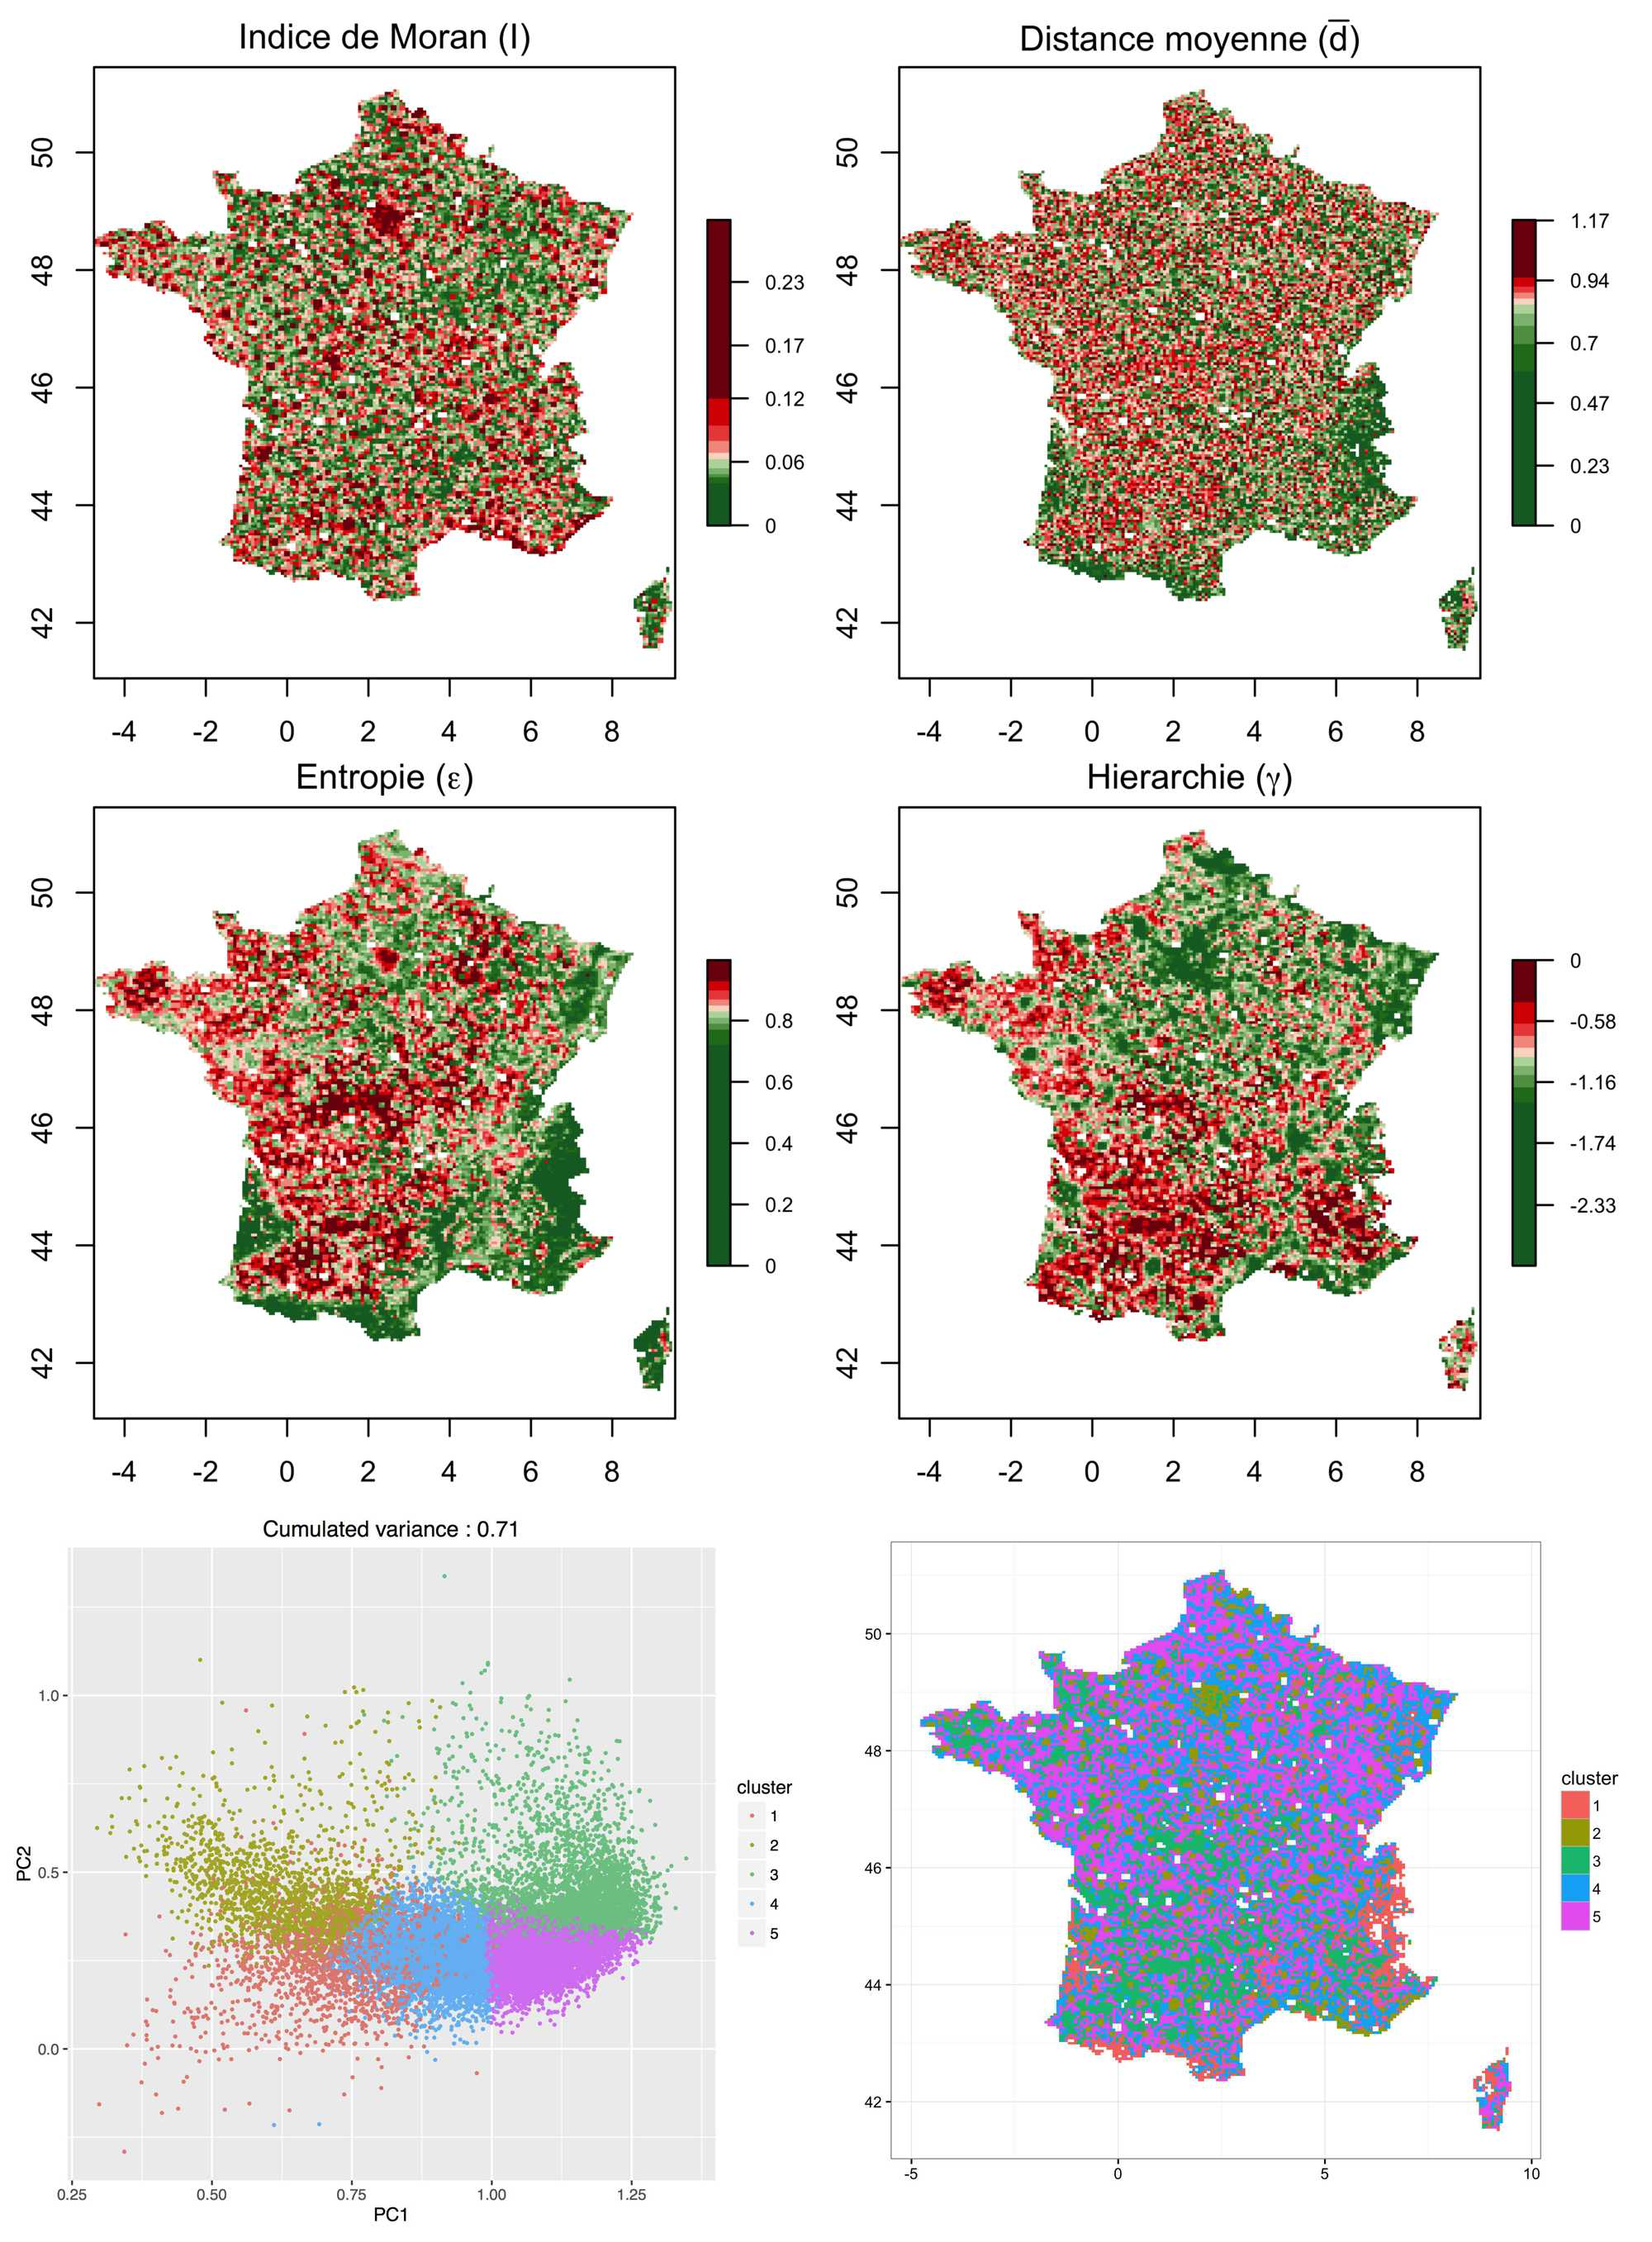
\includegraphics[width=0.9\linewidth]{Figures/Final/4-1-1-fig-staticcorrelations-empirical}
%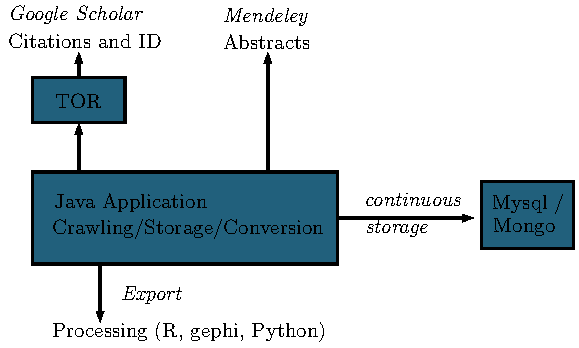
\includegraphics[width=0.9\linewidth]{Figures/Density/Fig1}
%\includegraphics[width=\textwidth]{figures/indics_morpho_discrquantiles}\\
%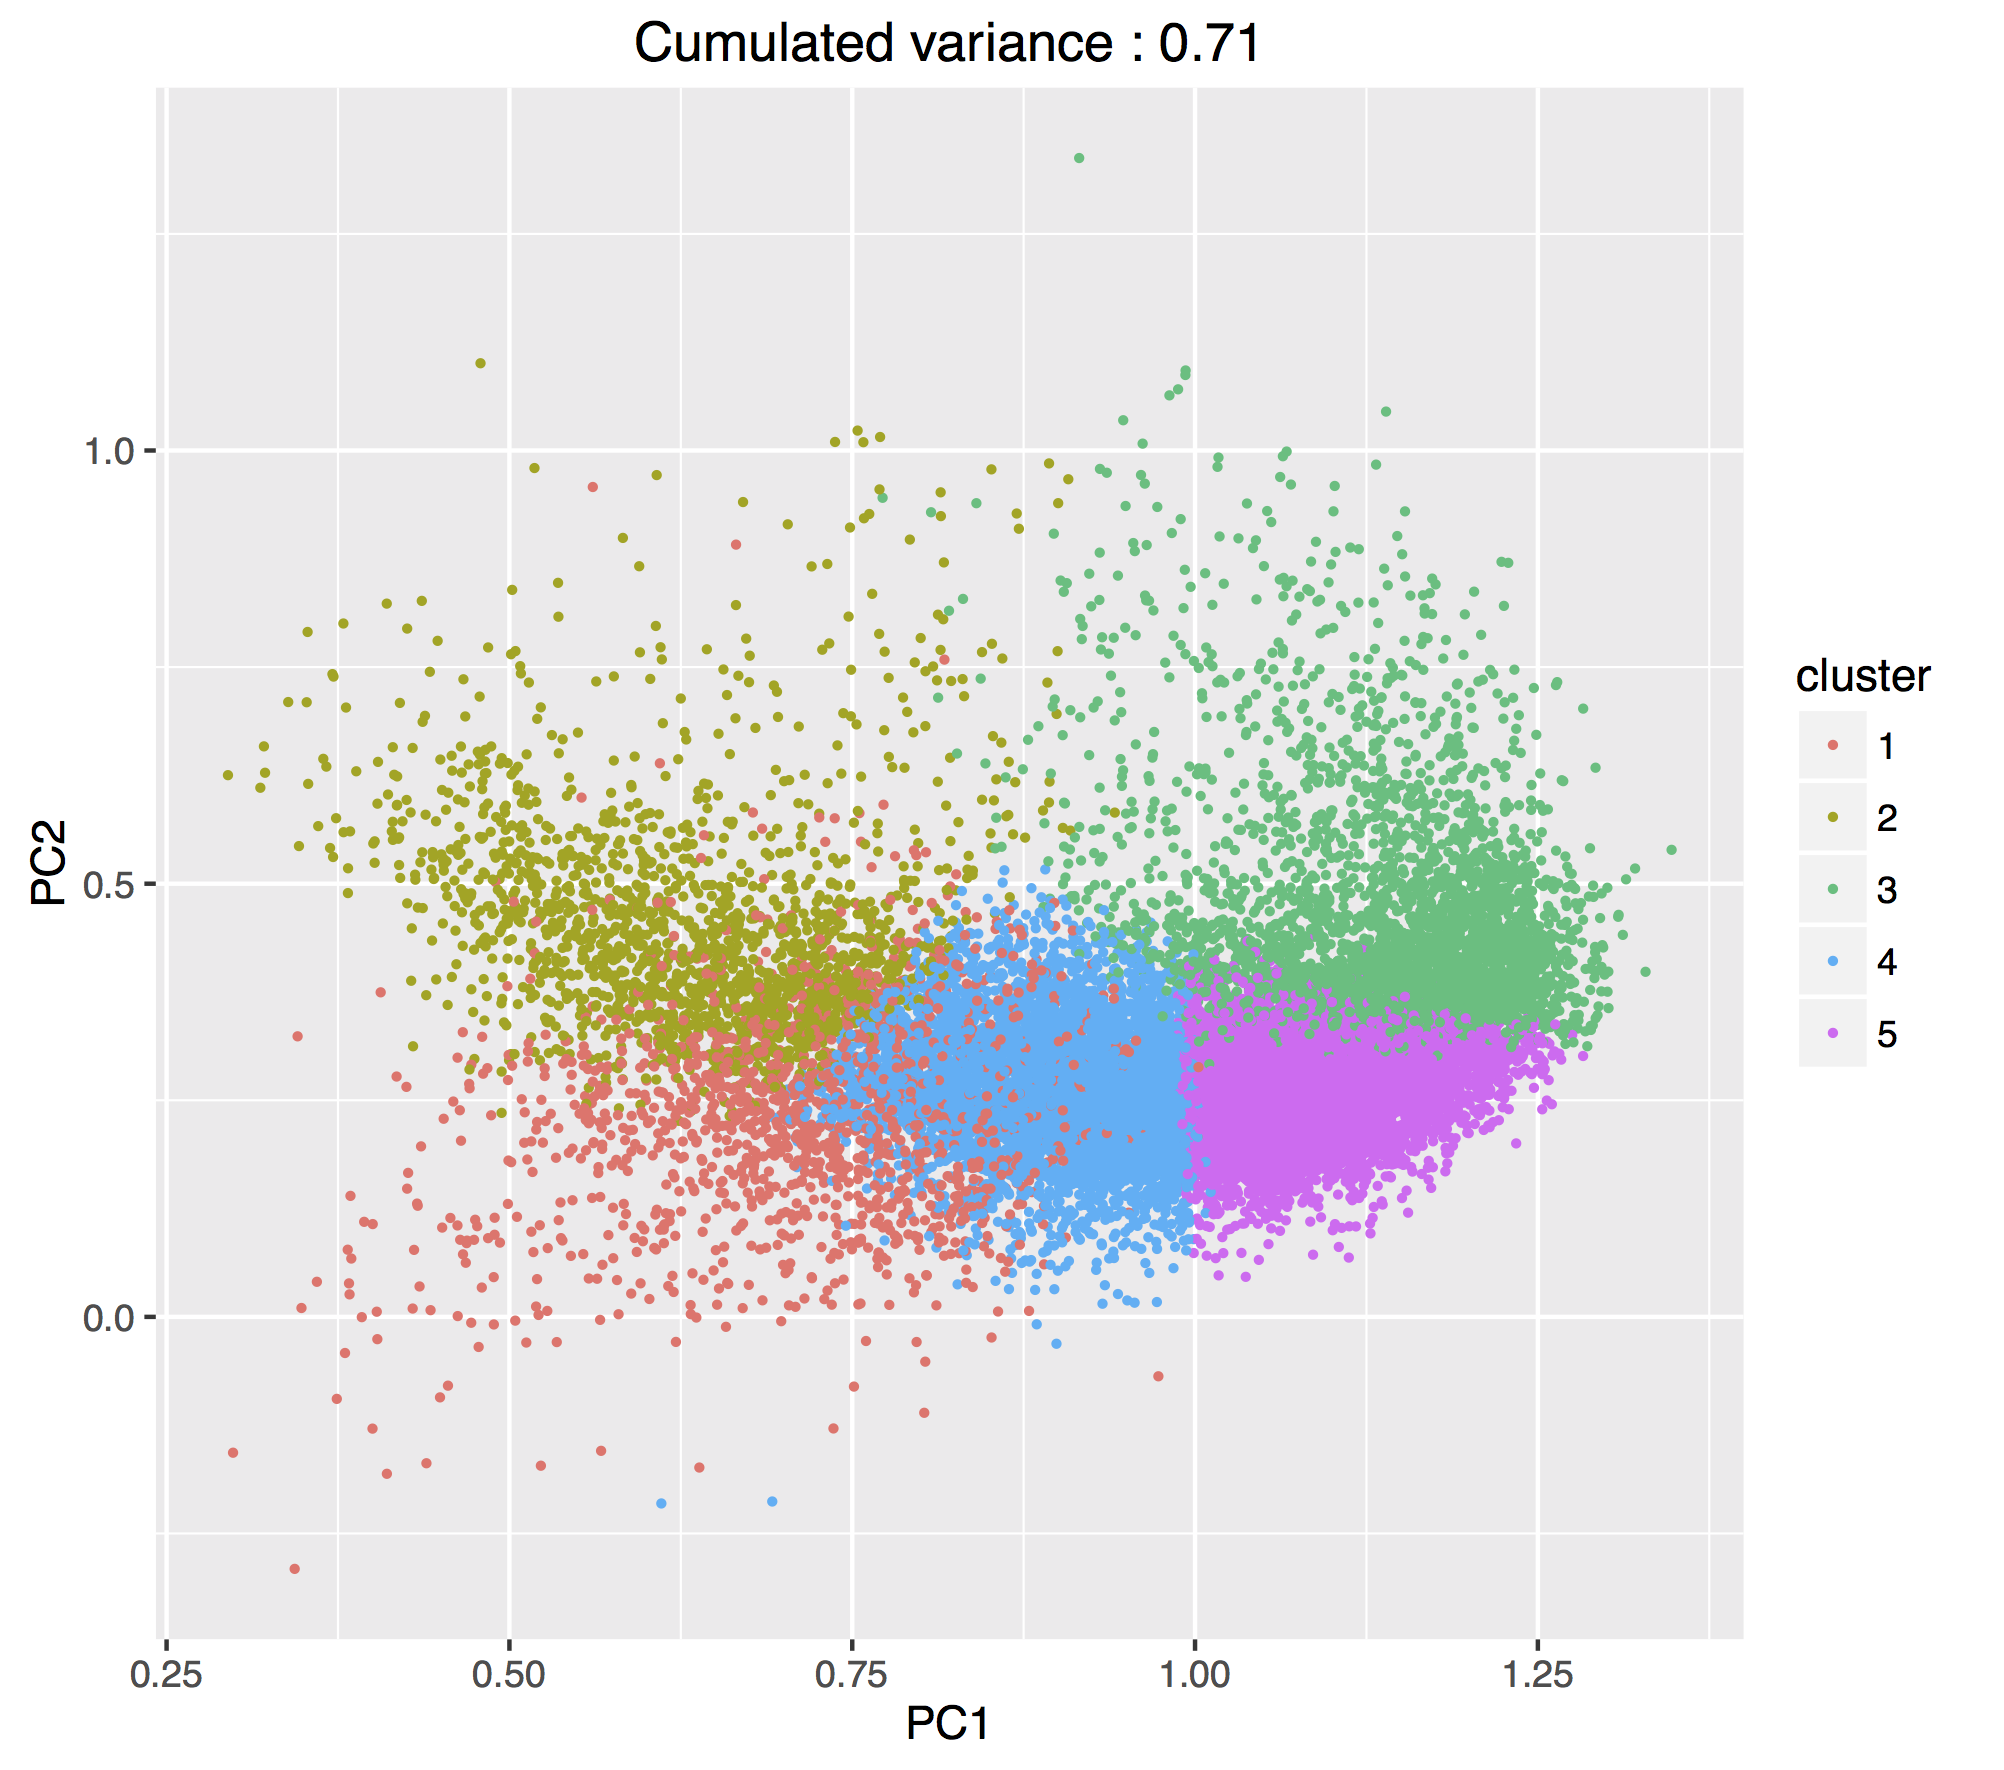
\includegraphics[width=0.49\textwidth]{figures/cluster_pca_k5_morpho}
%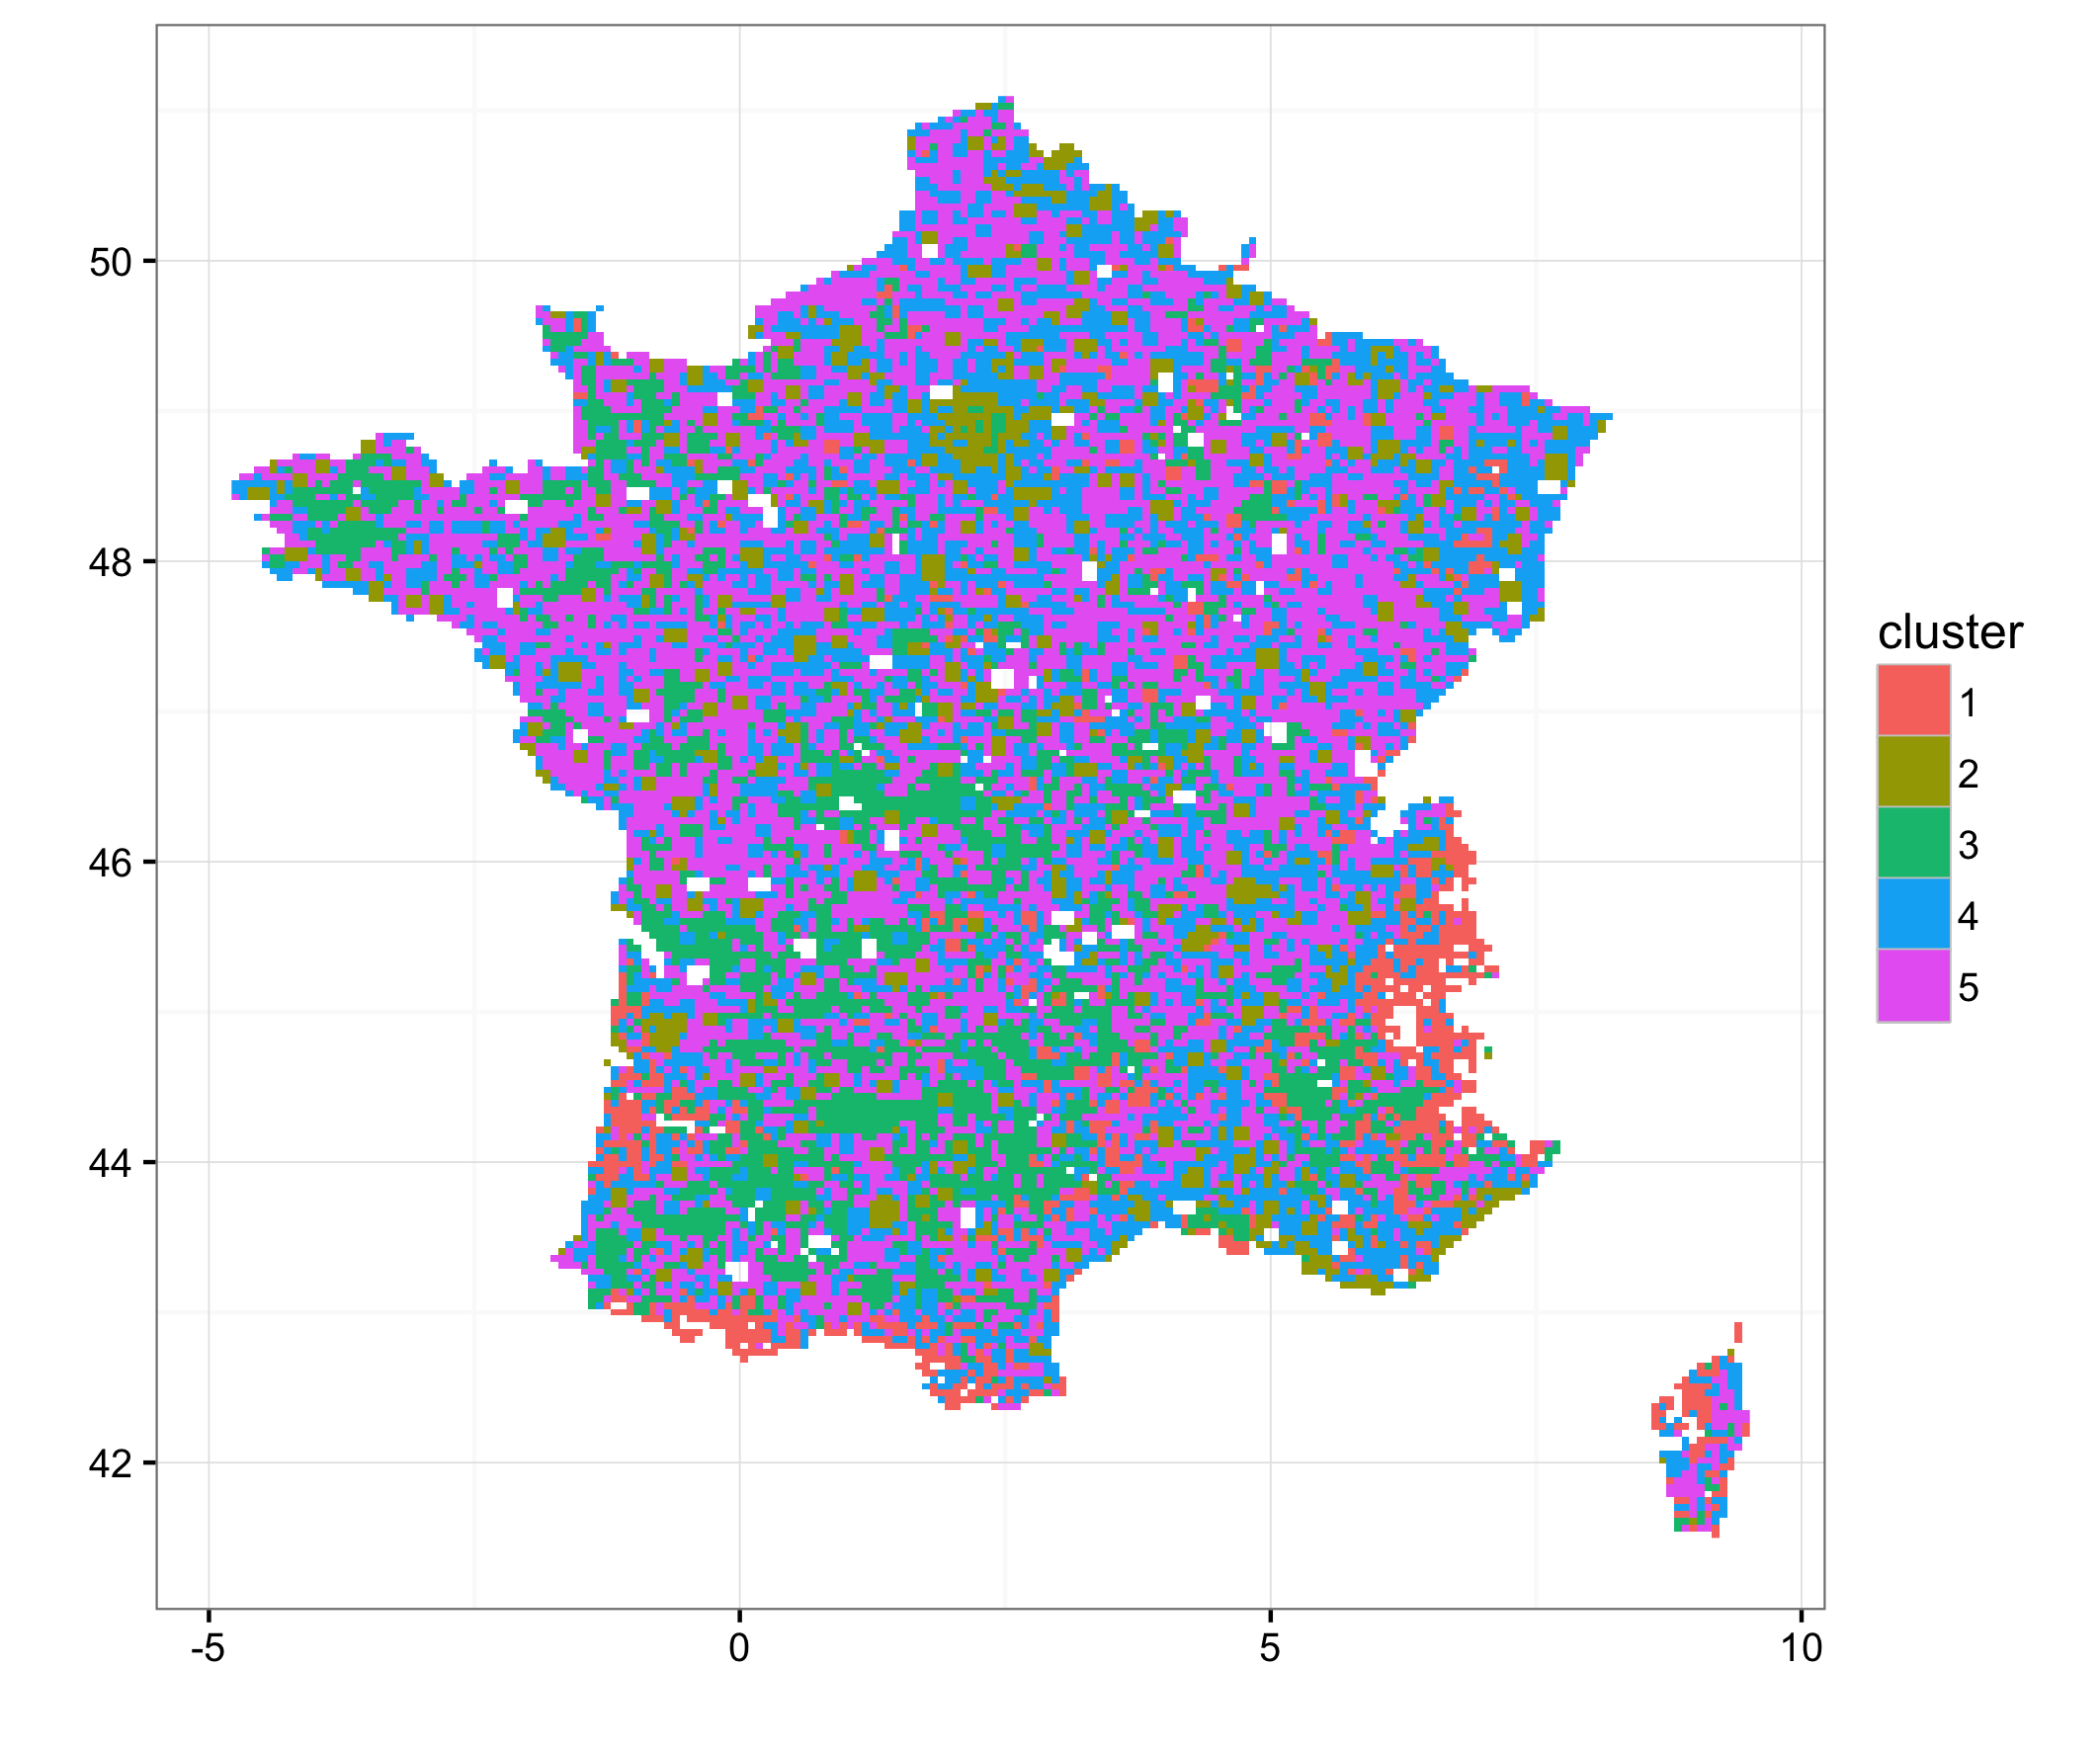
\includegraphics[width=0.49\textwidth]{figures/cluster_map_k5_morpho}
\caption[Empirical values of morphological indicators][Distribution spatiale des morphologies]{\textbf{Empirical values of morphological indicators.} \textit{(Top four maps)} Spatial distribution of the morphological indicators for France. Scale color discretization is done using quantiles to ease map readability. \textit{(Bottom Left)} Projection of morphological values on the two first components on a Principal Component analysis. Color gives cluster in an unsupervised classification (see text). \textit{(Bottom right)} Spatial distribution of clusters.\label{fig:staticcorrelations:empirical}}{\textbf{Valeurs empiriques des indicateurs morphologiques.} \textit{(Quatre cartes du haut)} Distribution spatiale des indicateurs morphologiques pour la France. La détermination de l'échelle de couleur est faite par quantiles pour faciliter la lecture des cartes. \textit{(Bas gauche)} Projection des valeurs morphologiques sur les deux premières composantes d'une analyse en composantes principales. La couleur donne le cluster dans une classification non supervisée (voir texte). \textit{(Bas droite)} Distribution spatiale des clusters. Se référer au texte pour les détails sur la procédure d'estimation spatiale des indicateurs et sur la procédure de classification.\label{fig:staticcorrelations:empirical}}
\end{figure}
%%%%%%%%%%%%%%%%%%%%%%%%

% \comment[FL]{tu n'indiques aucun nom de lieu. impossible a articuler avec le texte.}[c'est ecrit en francais, on espere que le lecteur sait situer Paris Lyon Marseille...]


\bpar{
We compute the morphological measures given above on real urban density data, using the population density grid of the European Union at 100m resolution provided openly by Eurostat~\cite{eurostat}. The choice of the resolution, the spatial range, and the shape of the window on which indicators are computed, is made according to the thematic specifications given before. We consider 50km wide square windows to be in accordance with the expected spatial range of one model instance. As it also does not make sense to have a too detailed resolution because of data quality, we take $N=100$ and aggregate the initial raster data at a 500m resolution to meet this size on real windows. To have a rather continuous distribution of indicators in space, we overlap windows by setting an offset of 10km between each, what also somehow rules out the question of window shape bias by the ``continuity'' of values. We tested the sensitivity to window size by computing samples with 30km and 100km window sizes and obtained rather similar spatial distributions.
}{
Nous calculons les mesures morphologiques données ci-dessus sur des données réelles de densité, en utilisant la grille de population de l'Union Européenne à la résolution de 100m fournie de manière ouverte par Eurostat~\cite{eurostat}\footnote{Cette base a certains défauts de précision qui ont été reconnus~\cite{bretagnolle2016ville} mais l'agrégation à une résolution supérieure devrait permettre de diminuer d'éventuels biais.}. Le choix de la résolution, de la portée spatiale, et de la forme de la fenêtre sur laquelle les indicateurs sont calculés, sont faits suivant les spécifications thématiques précédentes. Nous considérons des fenêtres carrées de largeur 50km. Comme une résolution trop détaillée n'est pas désirable à cause de la qualité des données\footnote{Selon \cite{batista2013high} qui détaille la construction du jeu de données, des bons résultats ont été obtenus après validation pour sept pays sur des échantillons avec une grille de résolution 1km. Nous nous rapprochons ainsi de cette résolution avec une grille de résolution 500m.}, nous agrégeons les données de la grille initiale à une résolution de 500m pour avoir des fenêtres de taille $N=100$ correspondant à 50km de côté. Pour obtenir une distribution des indicateurs relativement continue dans l'espace, nous superposons les fenêtres en posant un décalage de 10km entre chaque, ce qui induit un lissage des valeurs et permet de limiter les effets de bord dus à la forme. Nous avons par ailleurs testé la sensibilité à la taille de la fenêtre en calculant des échantillons avec des tailles de 30km et 100km et avons obtenu des distributions spatiales similaires, ainsi que de fortes corrélations entre les champs et leur lissage à une résolution plus fine, comme détaillé en Annexe~\ref{app:sec:staticcorrelations}.
}


\bpar{}{
L'implémentation des indicateurs doit être faite avec attention, puisque les complexités computationnelles peuvent atteindre $O(N^4)$ pour l'indice de Moran par exemple: nous utilisons la convolution par Transformée de Fourier Rapide, qui est une technique permettant de calculer l'indice de Moran avec une complexité en $O(\log^2 N \cdot N^2)$\footnote{C'est à dire ayant un temps d'execution borné par $\log^2 N \cdot N^2$ si $N$ est la taille des données, ce qui est un gain considérable par rapport à $N^4$ : pour le traitement d'une grille de côté 100, le facteur de gain asymptotique sera d'environ $10000$.}.
}

%Les distributions empiriques pour chaque indicateur sont données en Appendice~\ref{app:sec:staticcorrelations}. NON

\bpar{
We show in Fig.~\ref{fig:staticcorrelations:empirical} maps giving values of indicators for France only to ease maps readability. The first striking feature is the diversity of morphological patterns across the full territory. The auto-correlation is naturally high in Metropolitan areas, with the Parisian surroundings clearly detached. When looking at other indicators, it is interesting to denote regional regimes: rural areas have much less hierarchy in the South than in the North, whereas the average distance is rather uniformly distributed except for mountain areas. Regions of very high entropy are observed in the Center and South-West.
}{
Nous montrons en Fig.~\ref{fig:staticcorrelations:empirical} des cartes donnant les valeurs des indicateurs, pour la France seulement afin de permettre une lisibilité. La première caractéristique frappante est la diversité des motifs morphologiques au travers de l'ensemble du territoire. L'indice de Moran est relativement haut dans les zones englobant les métropoles (Paris, Lyon, Marseille par exemple), avec les environs de Paris qui se détachent clairement. Lorsqu'on s'intéresse aux autres indicateurs, il est intéressant, au regard de zones possibles dans laquelle une co-évolution peut s'opérer, de constater des régimes régionaux: les zones rurales ont beaucoup moins de hiérarchie dans le Sud que dans le Nord, tandis que la distance moyenne est plutôt distribuée uniformément sauf dans les zones montagneuses. Des régions qui présentent de fortes valeurs de l'entropie sont observées dans le centre et le Sud-ouest.
}

\bpar{
To have a better insight into morphological regimes, we use unsupervised classification with a simple k-means algorithm, for which the number of clusters $k=5$ witnesses a transition in inter-cluster variance. The split between classes is plotted in Fig.~\ref{fig:empirical}, bottom-left panel, where we show measures projected on the two first components of a Principal Component Analysis (explaining 71\% of variance). The map of morphological classes confirms a North-South opposition in a background rural regime (clear green against blue), the existence of mountainous (red) and metropolitan (dark green) regimes. Such a variety of settlements forms will be the target for the model. We did similar analysis for China using the gridded population data from~\cite{fu1km}: maps are available in~\ref{app:sec:staticcorrelations}.
}{
Pour avoir une meilleure compréhension des classes morphologiques existantes, nous utilisons une classification non-supervisée\footnote{Qui consiste à partitioner l'espace des données selon leur structure endogène.} avec un algorithme des k-means\footnote{Vu la distribution des points qui ont une densité relativement homogène, des méthodes alternatives comme l'algorithme DBScan sont relativement équivalentes. Nous prenons ici un nombre de répétitions $b=100$ de l'algorithme pour avoir un résultat robuste à la stochasticité.}. Le nombre de clusters $k=5$ induit une transition dans la variance inter-cluster, ce qui signifie qu'une variation de structure opère à ce nombre, que nous choisissons alors comme nombre de clusters. La séparation entre les classes est montrée en Fig.~\ref{fig:staticcorrelations:empirical}, panneau bas gauche, où nous représentons les mesures projetées sur les deux premières composantes d'une Analyse en Composantes Principales (expliquant 71\% de la variance, ce qui est relativement conséquent). La carte des classes morphologiques confirme une opposition Nord-Sud dans le régime rural de fond (vert clair contre bleu), l'existence d'un régime de montagne (rouge) et d'un régime métropolitain (vert sombre). Une telle variété d'établissements sera l'un des objectifs du modèle en~\ref{sec:densitygeneration}. Un calcul similaire des indicateurs morphologiques a été effectué pour la Chine en utilisant la grille de population à 1km fournie par~\cite{fu1km}. Les cartes sont disponibles en Appendice~\ref{app:sec:staticcorrelations}.
}


% \comment{\cite{goerlich2017clustering} : variable prises en compte, ne pas prendre pop sinon catégories pas intéressantes comme ce papier}

%%%%%%
% Correlation entre 50km smoothé et 100km (idem 30km) pour quantifier sensibilite a la taille de la fenetre. forme : calcul de coin de table avec smoothing.
% -> cf appendice sur sensitivity a la resolution






%%%%%%%%%%%%%%%%%%
\subsection{Network Measures}{Mesures de Réseau}


\bpar{
We consider network aggregated indicators as a way to characterize transportation network properties on a given territory, the same way morphological indicators yielded information on urban structure. We propose to compute some simple indicators on same extents as for morphology, to be able to explore relations between these static measures.
}{
Nous considérons d'autre part les mesures agrégées de réseau comme un moyen de caractériser les propriétés des réseaux de transport sur un territoire donné, de la même façon que les indicateurs morphologiques informent sur la structure urbaine. Nous proposons de calculer des indicateurs simples sur des étendues spatiales similaires à celles retenues pour la mesure de la morphologie, pour être en mesure d'explorer les relations entre ces mesures statiques.
}

\bpar{
Static network analysis has been extensively documented in the literature, see for example \cite{louf2014typology} for a cross-sectional study of cities or \cite{2015arXiv151201268L} for exploration of new measures for the road network.
}{
L'analyse statique de réseau a été intensément documentée dans la littérature, voir par example \cite{louf2014typology} pour une étude comparative des villes ou \cite{2015arXiv151201268L} pour l'exploration de nouvelles mesures pour le réseau de rues. \cite{2017arXiv170902939M} utilise des techniques issues de l'apprentissage profond pour établir une typologie des réseaux viaires urbains pour un grand nombre de villes dans le monde.
}

\bpar{
}{
Les enjeux derrière ce genre d'approches sont multiples : elles peuvent viser à des typologies ou caractérisations de réseaux spatiaux, à des compréhensions des processus dynamiques sous-jacents dans un but de modélisation de la morphogenèse, ou même de planification urbaine comme sont appliquées parfois les approches par \emph{Space Syntax}~\cite{hillier1989social}. Nous nous plaçons ici plutôt dans les deux premières logiques puisque nous cherchons à caractériser la forme des réseaux dans un premier temps, puis d'inclure leur dynamique dans des modèles dans un second temps. Notre contribution significative est la caractérisation du réseau routier sur de grandes étendues spatiales, couvrant l'Europe et la Chine.
}


\subsubsection{Indicators}{Indicateurs}

\bpar{
These indicators are used to capture a rough picture of the structure. Refined work at smaller scales (intra-urban road network) and with more elaborated measures that allow to differentiate more precisely local form, was recently done by Lagesse in~\cite{2015arXiv151201268L}.
Network macroscopic structure is summarized by the following set of indicators, after the simplifications and reductions done in the previous step. Assuming network given by $N=(V,E)$, nodes spatial positions $\vec{x}(V)$ and edges \emph{effective distances} $d(E)$ taking into account impedances and real distances (to include basically network hierarchy), we have indicators:
}{
Nous introduisons des indicateurs pour avoir une idée large de la forme du réseau, utilisant un certain nombre d'indicateurs pour capturer le maximum de dimensions des propriétés des réseaux, plus ou moins liées à l'utilisation de ceux-ci. Ces indicateurs résumant la structure mesoscopique du réseau sont calculés sur les réseau topologiques obtenus par les étapes précédentes de simplification. Notant le réseau $N=(V,E)$, les noeuds $V$ ont des positions spatiales $\vec{x}(v)$ et des populations $p(v)$ obtenues par agrégation de la population dans le polygone de Voronoï correspondant\footnote{Un diagramme de Voronoï est une partition du plan, formée à partir d'un nuage de point. La cellule associée à chaque point est constituée de l'ensemble des points plus proches de celui-ci que des autres points du nuage. Le graphe d'un diagramme de Voronoï est le dual de celui de la triangulation de Delaunay associée.}, les liens $E$ ont des \emph{distances effectives} $l(E)$ qui prennent en compte les impédances et les distances réelles (pour inclure la hiérarchie primaire du réseau). Nous utilisons alors :
}

%"vcount"      "ecount" "gamma"   "meanDegree"   "mu"  "alpha"        "meanLinkLength"     "meanNodePop"        "meanClustCoef"      "components"        "meanBetweenness"    "alphaBetweenness"   "euclPerf"           "diameter"        "meanCloseness"      "alphaCloseness.x"   "meanTravelTime"     "alphaTravelTime.x"  "alphaAccessibility" "meanAccessibility"  "modularity"

\bpar{
\begin{itemize}
\item connectivity
\item degree distribution
\item centrality, taken as normalized mean \emph{betweenness-centrality}
\item average path length
\item network diameter
\item mean network speed
\end{itemize}
}{
\begin{itemize}
\item Caractéristiques du graphe, issues de la théorie des graphes, comme définies par~\cite{haggett1970network} : nombre de noeuds $\left|V\right|$, nombre de lien $\left|E\right|$, densité $d$, longueur moyenne des liens $\bar{d_l}$, coefficient de clustering moyen $\bar{c}$, nombre de composantes $c_0$.
\item Mesures liées au plus courts chemins : diamètre $r$, performance euclidienne $v_0$ (définie par~\cite{banos2012towards}), longueur moyenne des plus courts chemins $\bar{l}$.
\item Mesures de centralité : celles-ci sont agrégées au niveau du réseau en prenant leur moyenne et leur niveau de hiérarchie, calculé par un ajustement des moindres carrés d'une loi rang taille, pour les mesures de centralité suivantes :
\begin{itemize}
\item Centralité d'intermédiarité~\cite{crucitti2006centrality}, moyenne $\bar{bw}$ et hiérarchie $\alpha_{bw}$ : étant donné la distribution de la centralité sur l'ensemble des noeuds, on prend la pente d'un ajustement rang-taille ainsi que la moyenne de la distribution.
\item Centralité de proximité~\cite{crucitti2006centrality}, moyenne $\bar{cl}$ et hiérarchie $\alpha_{cl}$
%\item Temps de trajet moyen vers les autres noeuds, moyenne $\bar{t}$ et hiérarchie $\alpha_{t}$ (prend en compte la vitesse maximale des liens) % pas utilisé finalement
\item Accessibilité~\cite{hansen1959accessibility}, qui est dans notre cas calculée comme une centralité de proximité pondérée par les populations : moyenne $\bar{a}$ et hiérarchie $\alpha_{a}$
\end{itemize}
%\item Modularité~\cite{blondel2008fast}, qui exprime la structure en communautés du réseau.
% , population moyenne $\bar{p}$ degré moyen $\bar{\delta}$ , nombre cyclotomique $\mu$  connectivité $\alpha$, 
\end{itemize}
}

Le concept d'accessibilité est mesuré ici par un indicateur de réseau, puisque son calcul implique d'attribuer des poids aux noeuds avec une population correspondante, et peut être interprété ensuite comme un potentiel d'accès au reste de la population (comme nous l'avons fait en Chapitre~\ref{ch:thematic}). Cet indicateur est a priori intéressant car à l'interface entre forme urbaine et forme du réseau, puisque la distribution de population sur les noeuds est prise en compte.

La performance du réseau est proche de la mesure de rectilinéarité (\emph{straigthness}) proposée par \cite{josselin2016straightness}, qui montre qu'elle différencie efficacement réseaux rectilinéaires et réseaux radio-concentriques, réseaux urbains récurrents.

Nos indicateurs sont conçus autour de la topologie du réseau mais pas son usage : des développements avec les données appropriées peuvent étendre ces analyses à l'aspect fonctionnel des réseaux, comme par exemple des mesures de performance calculées par~\cite{trepanier2009calculation} par l'intermédiaire de données massives pour un réseau de transports en commun.



%%%%%%%%%%
%% -- ON HOLD -- (HS)

%\subsubsection{Network Shape and Resilience}{Forme de Réseau et Résilience}
%L'idée fondamentale motivant le calcul d'indicateurs de réseau est d'obtenir une réduction de dimension drastique, s'il est possible d'associer certains ``types'' de réseau à des valeurs typiques d'indicateurs. On est très loin d'une connaissance fine de typologies qui associeraient propriétés topologiques, dynamiques et processus de génération du réseau, le tout de manière synthétique. Il est de même difficile de relier systématiquement ces propriétés à des caractéristiques dérivées, comme par exemple pour la résilience qui est une propriété aux définitions diverses\footnote{Pour laquelle~\cite{Gao:2016ty} introduit une nouvelle approche par la sensibilité des processus dynamiques.}. Afin d'illustrer d'une part la difficulté de caractériser les réseaux et d'autre part les potentialités offertes par notre base de données, nous développons en Appendice~\ref{app:sec:staticcorrelations} une courte analyse des propriétés de résilience au sens de~\cite{ash2007optimizing} pour des réseaux typiques. Cette analyse fait, de la même manière que le calcul des indicateurs, partie d'une démarche générale de caractérisation des réseaux, essentielle ici comme préliminaire à l'étude de leur interaction avec les territoires.




\subsubsection{Data preprocessing}{Pré-traitement des données}


\bpar{
We work here with the road network, which structure is finely conditioned to territorial configuration of population densities. Furthermore, data for present day road network is openly available through the OpenStreetMap project~\cite{openstreetmap}. Its quality was investigated for different countries such as England~\cite{haklay2010good} and France~\cite{girres2010quality}. It was found to be of a quality equivalent to official surveys for the primary road network. Concerning China, although \cite{zheng2014assessing} underlined a quick acceleration of OpenStreetMap road data completeness and accuracy, its use for computation of network indicators may be questioned at a very fine scale. \cite{zhang2015density} highlights four regimes of data quality, partitioning China into regions among which qualitative behavior of OSM data varies. We underline that the results will be more valid on the regions where the quality is the highest, i.e. with high density and high diversity.
}{
Nous travaillons ici avec le réseau de rues, dont la structure est finement conditionnée aux configurations territoriales des densités de population. De plus, les données du réseau de routes actuel est disponible ouvertement par l'intermédiaire du projet OpenStreetMap (OSM)~\cite{openstreetmap}. Sa qualité a été étudiée pour différents pays comme l'Angleterre~\cite{haklay2010good} et la France~\cite{girres2010quality}. Il a été établi pour ces pays une qualité équivalente aux données officielles pour le réseau de rues primaire, au sens à la fois de la couverture spatiale et de la précision locale. Dans le cas de la Chine, bien que \cite{zheng2014assessing} soulève une récente accélération de la couverture et de la précision des données OSM pour les routes, leur usage pour le calcul d'indicateurs de réseau peut être questionné à une échelle très fine. \cite{zhang2015density} fournit une partition de la Chine en régions entre lesquelles le comportement qualitatif des données OSM varie. Nous devrons garder à l'esprit cette variabilité, et pour être assuré de la fiabilité des résultats, nous simplifierons le réseau à un niveau d'agrégation suffisant.
}




\bpar{
From the primary road segments, we compute the topological road network for all studied areas, at 100m granularity scale to be used consistently with the population grid. The OSM data is imported into \texttt{pgsql} using \texttt{osmosis}, is then aggregated at fixed granularity, and the resulting topological network is finally simplified with a split/merge algorithm. We have for Europe $\simeq 44\cdot 10^6$ links in initial OSM db, $\simeq 61\cdot 10^6$ in first simplified layer, $\simeq 21\cdot 10^6$ in final database. For a given dataset corresponding to a subset of the overall road network, it is necessary to simplify network structure by spatial aggregation as initial data presents very detailed features and thus a very large numbers of nodes ($\simeq 10^10$ for Europe dataset). It is possible to drastically reduce network size by spatial aggregation of nodes and link replacements. The detailed algorithm and implementation are detailed in Supplementary material~\ref{app:sec:staticcorrelations}.
}{
Le réseau constitué des segments de rue primaires est agrégé à la granularité fixe de la grille de densité pour créer un graphe. Celui-ci est ensuite simplifié pour garder uniquement la structure topologique du réseau, les indicateurs normalisés étant relativement robustes à cette opération. Celle-ci est nécessaire pour un calcul simple des indicateurs et une cohérence thématique avec la couche de densité. On garde uniquement les noeuds ayant un degré strictement supérieur ou inférieur à deux, et les liaisons correspondantes, en prenant soin d'agréger la distance géographique réelle en construisant le lien topologique correspondant. Vu l'ordre de grandeur de taille des données (pour l'Europe, la base initiale a $\simeq 44.7\cdot 10^6$ liens, et la base finale simplifiée $\simeq 20.4\cdot 10^6$), un algorithme spécifique parallèle est mis en place, de structure \emph{split-merge}. Celui-ci découpe l'espace en zones qui peuvent être traitées indépendamment puis fusionnées. Il est détaillé en Appendice~\ref{app:sec:staticcorrelations}.
}



%china 2048589 ; simpl 2022802
%europe 44706945 ; simpl 20443061






\subsubsection{Results}{Résultats}


\bpar{}{
Les indicateurs de réseau ont été calculés sur les mêmes zones que les indicateurs de forme urbaine, pour pouvoir les mettre en correspondance directe et calculer les correlations par la suite. Nous montrons en Fig.~\ref{fig:staticcorrs:network} un échantillon pour la France.
}

\bpar{}{
Le comportement spatial des indicateurs révèle comme pour la forme urbaine des régimes locaux (urbain, rural, métropolitain), mais aussi des régimes régionaux très marqués. Ceux-ci peuvent être dus aux différentes pratiques agricoles selon les régions dans le cas du rural par exemple, impliquant une partition différente des parcelles ainsi qu'une organisation particulière de leur desserte. En taille du réseau, la Bretagne se détache nettement et rejoint les régions urbaines, témoignant de parcelles très fragmentées (et a fortiori d'un découpe foncière fragmentée également dans l'hypothèse simplificatrice d'une coincidence des parcelles et du foncier). Cela est partiellement corrélé à une faible hiérarchie dans l'accessibilité. Le Sud et l'Est du Bassin Parisien étendu se distinguent par une forte centralité d'intermédiarité moyenne, en accord avec une forte hiérarchisation du réseau.
}

De la même manière que pour la forme urbaine, cette variabilité spatiale suggère la recherche de régimes variables d'interaction entre indicateurs, comme nous le ferons plus loin par l'intermédiaire de leur corrélations.


\bpar{}{
Pour la Chine, pour laquelle une selection d'indicateurs est également donnée en~\ref{app:sec:staticcorrelations}, on observe des variations locales et régionales encore plus marquées. Les zones urbaines fortement peuplées se détachent, correspondant à un régime bien particulier.
}


L'indicateur d'accessibilité est finalement fortement corrélé au même non-pondéré, c'est à dire la centralité de proximité : nous obtenons une corrélation de $\rho = 0.86$ estimée sur l'ensemble des points de mesure pour la Chine.


%%%%%%%%%%%%%%%%%%%%%%%%
\begin{figure}
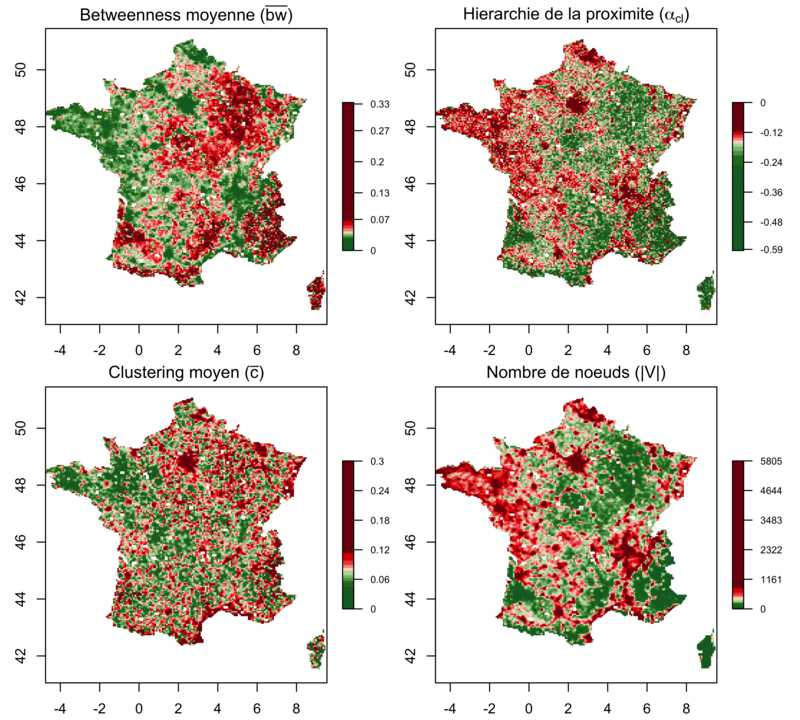
\includegraphics[width=\linewidth]{Figures/Final/4-1-2-fig-staticcorrs-network}
%\includegraphics[width=\linewidth]{Figures/StaticCorrelations/FR_indics_network_selected_2_discrquantiles}
\caption[Empirical values of network indicators][Distribution spatiale des indicateurs de réseau]{\textbf{Empirical values of network indicators.}\label{fig:staticcorrs:network}}{\textbf{Distribution spatiale des indicateurs de réseau.} Nous calculons les indicateurs pour la France, en correspondance avec les indicateurs morphologiques décrits précédemment. Nous donnons ici la centralité de chemin moyenne $\bar{bw}$, la hiérarchie de la centralité de proximité $\alpha_{cl}$, le coefficient de clustering moyen $\bar{c}$ et le nombre de noeuds $\left|V\right|$.\label{fig:staticcorrs:network}}
\end{figure}
%%%%%%%%%%%%%%%%%%%%%%%%




%%%%%%%%%%%%%%%%%%
\subsection{Effective static correlations}{Correlations Statiques Effectives et Non-stationnarité}



%%%%%%%%%%%%%%%%%%
\subsubsection{Spatial Correlations}{Corrélations spatiales}


\bpar{
Pour les correlations : zones de correlation pas trop grandes, carrés de base indicateurs plus petits : Computation of urban form indicators~\cite{le2015forme} and network indicators on $l_0=10km$ side square. Computation of spatial correlation on square areas of width $\delta\cdot l_0$ (with typically $\delta = 4, \ldots , 16$) We clearly unveil the local spatial stationarity of processes.
}{
Les corrélations spatiales locales sont calculées sur des fenêtres regroupant un certain nombre d'observation, et donc de fenêtres sur lesquelles les indicateurs ont été calculés. Notons $l_0$ (qui vaut 10km dans les résultats précédents) la résolution des distributions des indicateurs. L'estimation des corrélations s'effectue alors sur des carrés de taille $\delta\cdot l_0$ (avec $\delta$ pouvant varier typiquement de 4 à 100). $\delta$ donne à la fois le nombre d'observations utilisées pour l'estimation locale de la corrélation, et la portée spatiale de la fenêtre correspondante. Sa valeur influe donc directement la fiabilité de l'estimation.
}

\bpar{}{
Nous montrons en Fig.~\ref{fig:staticcorrs:mapscorrs} des exemples de corrélations estimées avec $\delta = 12$ dans le cas de la France. Avec 20 indicateurs, la matrice de corrélation est assez conséquente en taille, mais la dimension effective (le nombre de composantes nécessaires pour atteindre la majorité de la variance) est réduite : une analyse en composante principale montre que 10 composantes capturent 62\% de la variance, et la première composante capture déjà 17\%, ce qui est considérable dans un espace où la dimension est de 190\footnote{Il s'agit de la dimension de la matrice de correlation entre 20 indicateurs, c'est à dire le nombre d'éléments de sa moitié moins sa diagonale. Si les corrélations étaient distribués aléatoirement, la première composante capturerait $1/190 = 0.5\%$ seulement, et les 10 premières 5\%, puisque la variance se répartit équitablement entre des dimensions indépendantes.}.
}



\bpar{}{
Il est possible d'examiner le sous-bloc pour la forme urbaine, pour le réseau, ou les corrélations croisées, qui expriment directement un lien entre les propriétés de la forme urbaine et celles du réseau. Par exemple, la relation entre centralité de chemin moyenne et hiérarchie morphologique que l'on visualise permet de comprendre la processus correspondant à la correspondance des hiérarchies : une population hiérarchisée peut induire un réseau hiérarchisé ou le sens inverse, mais elle peut également induire un réseau distribué ou celui-ci peut créer une hiérarchie de population - il faut bien comprendre en terme de correspondance et non de causalité, mais cette correspondance informe sur différents régimes urbains. Les métropoles semblent présenter une corrélation positive pour ces deux indicateurs, comme le montre la Fig.~\ref{fig:staticcorrs:mapscorrs}, et des espaces ruraux une corrélation négative.
}



\bpar{}{
Afin de se donner une idée des relations globales entre indicateurs, on peut se référer à la matrice de corrélation complète en Fig.~\ref{fig:app:staticcorrelations:overallcorrs} (Annexe~\ref{app:sec:staticcorrelations}) : par exemple, une forte hiérarchie de population est liée à une centralité de chemin forte et hiérarchisée, mais est corrélée négativement au nombre de sommets (une population diffuse nécessite un réseau plus maillé pour la desserte). Toutefois, il n'est pas possible ainsi de systématiquement lier les indicateurs, puisque ceux-ci varient justement fortement dans l'espace. Nous donnons également en Annexe~\ref{app:sec:staticcorrelations}, Fig.~\ref{fig:app:staticcorrelations:europe-correlations}, des cartes de différents coefficients de corrélation pour l'ensemble de l'Europe. 
}



\bpar{}{
Cela suggère une très grande variété de régimes d'interaction. La variation spatiale de la première composante de la matrice réduite confirme celle-ci, ce qui révèle clairement la non-stationnarité spatiale des processus d'interaction entre formes, puisque les premiers et second moments varient dans l'espace. La significativité statistique de la non-stationnarité spatiale peut être vérifiée de différentes façons\footnote{Il n'existe à notre connaissance pas de test générique de non-stationnarité spatiale. \cite{zhang2014test} développe par exemple un test pour des régions rectangulaires de dimensions quelconques, mais dans le cas spécifiques des \emph{point processes}.}. Nous utilisons ici la méthode de \cite{leung2000statistical} qui consiste à estimer par bootstrap la robustesse de modèles de Régression Géographique Pondérée. Ceux-ci seront développés ci-dessous, mais on obtient pour l'ensemble des modèles testés une non-stationnarité significative sans équivoque ($p<10^{-3}$).
}





% -- eventuellement ajout test de stationnarité ici --
%  -> test avec GWR


Par ailleurs, la distribution statistique des corrélations donnée en Fig.~\ref{fig:app:staticcorrelations:corr-distribs}  en Annexe~\ref{app:sec:staticcorrelations} suit une loi asymétrique pour la morphologie seule, et plutôt symétrique pour le réseau et le croisement, ce qui voudrait dire que certaines zones ont des contraintes morphologiques assez fortes tandis que la forme du réseau est plutôt libre. Enfin, on constate sur les nuages de points de la même figure, croisant les valeurs des corrélations dans les différents blocs, que les configurations où les corrélations croisées sont les plus fortes correspondent à celles où les corrélations morphologiques et de réseau sont également fortes, confirmant l'imbrication des processus dans ce cas.


%%%%%%%%%%%%%%%%%%%%%%%%
\begin{figure}[h!]
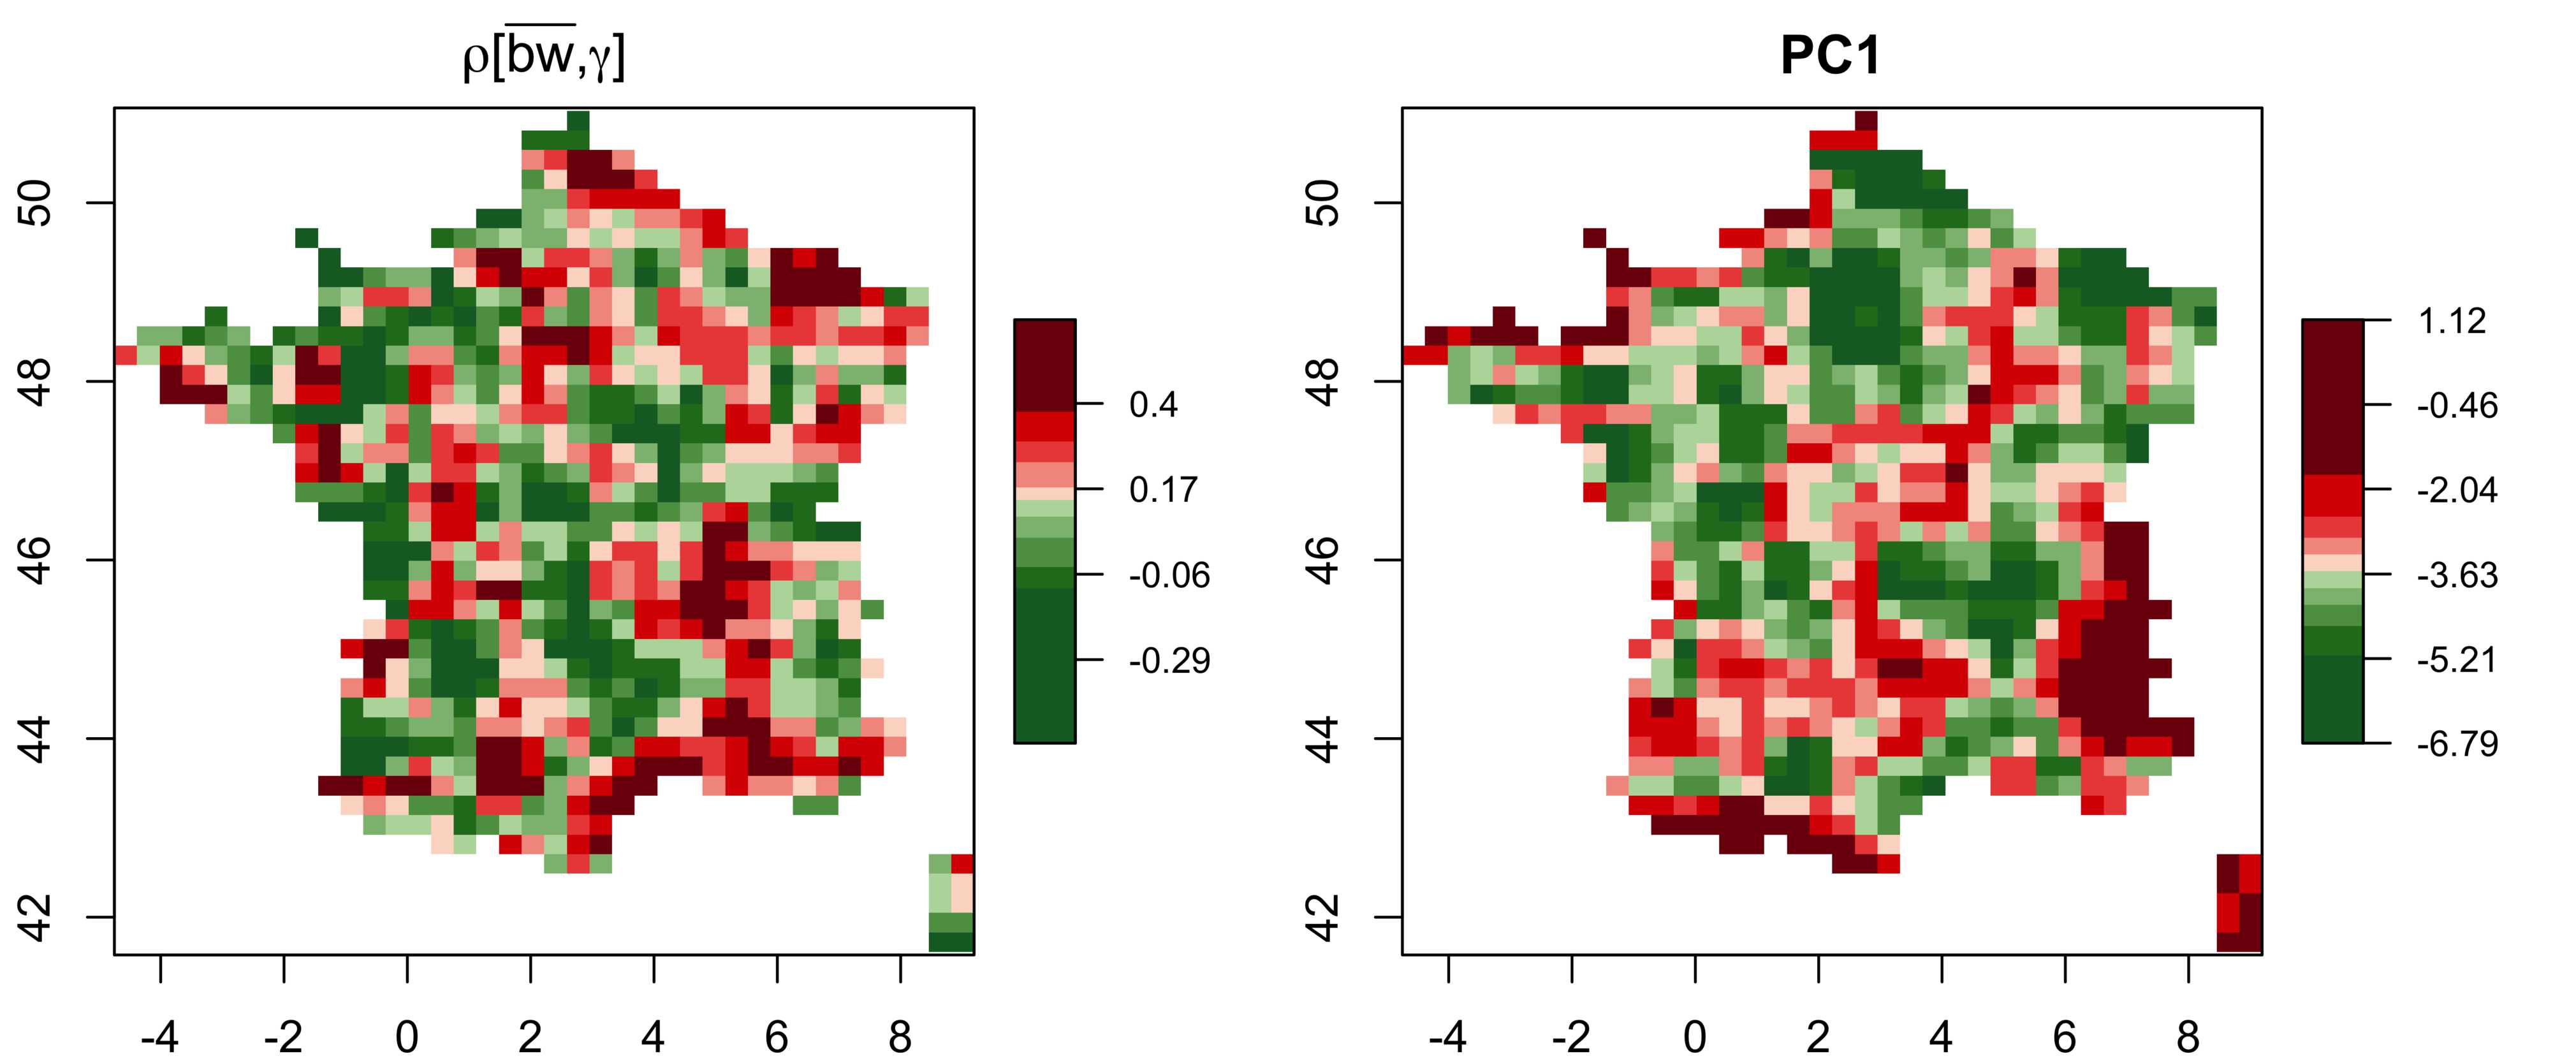
\includegraphics[width=\linewidth]{Figures/Final/4-1-3-fig-staticcorrs-mapscorrs}
%\includegraphics[width=0.48\linewidth]{Figures/StaticCorrelations/FR_corr_meanBetweenness_slope_rhoasize12}
%\includegraphics[width=0.48\linewidth]{Figures/StaticCorrelations/FR_corr_PCA_rhoasize12}
\caption[Spatial Correlations][Corrélations Spatiales entre indicateurs morphologiques et indicateurs de réseau]{Spatial Correlations\label{fig:staticcorrs:mapscorrs}}{\textbf{Exemples de corrélations spatiales.} Pour la France, les cartes donnent $\rho\left[\bar{bw},\gamma\right]$, corrélation entre la centralité de chemin moyenne et la hiérarchie de la population (\textit{Gauche}) et la première composante de la matrice réduite (\textit{Droite}).\label{fig:staticcorrs:mapscorrs}}
\end{figure}
%%%%%%%%%%%%%%%%%%%%%%%%



%%%%%%%%%%%%%%%%%%
\subsubsection{Variations of the estimated correlations}{Variations des corrélations estimées}


\bpar{
$\rightarrow$ Significant variation of mean correlation with $\delta$ (Left) and of normalized confidence interval (Right) given by $\left|\rho_+ - \rho_-\right|\cdot \delta$, as bounds theoretically vary as $\sqrt{N} \sim \sqrt{\delta^2}$ : implies multi-scalarity
}{
Nous montrons en Fig.~\ref{fig:staticcorrs:corrsdistrib} la variation de l'estimation des corrélations en fonction de la taille de la fenêtre. Plus précisément, on observe une forte variation des correlations en fonction de $\delta$, qui se reflète dans la valeur moyenne de la matrice donnée ici (s'étendant par exemple de $\rho(4)=0.22$ à $\rho(80)=0.12$ pour les corrélations croisées absolues moyennes). L'augmentation de $\delta$ cause pour l'ensemble un décalage dans le positif, mais également un rétrécissement de la distribution, ces deux effets se traduisant par une décroissance des corrélations absolues moyennes, qui se stabilisent approximativement pour les grandes valeurs de $\delta$. Cette variation pourrait être révélatrice d'un comportement multi-échelle : le changement de la taille de la fenêtre ne devrait pas influer l'estimateur si un seul processus était sous-jacent, elle devrait seulement changer la robustesse de l'estimation. Le développement en Annexe~\ref{app:sec:staticcorrelations} illustre ce lien dans le cas de processus superposés à deux échelles, et démontre que cette structure de processus implique une variation de la corrélation estimée en fonction de $\delta$, au moins dans les faibles valeurs, ce que nous observons ici en Fig.~\ref{fig:staticcorrs:corrsdistrib}.
}



\bpar{}{
Par ailleurs, la variation de la taille normalisée de l'intervalle de confiance pour les corrélations, qui en théorie sous hypothèse de normalité devrait conduire $\delta\cdot \left|\rho_+ - \rho -\right|$ à être constant, puisque les bornes varient asymptotiquement comme $1/\sqrt{N}\sim 1/\sqrt{\delta^2}$ (la démonstration est donnée en Appendice~\ref{app:sec:staticcorrelations}), va dans la direction de cette hypothèse de processus superposés à plusieurs échelles comme proposé précédemment.
}


Ainsi, les processus sont à la fois non-stationnaires, et des indices poussent à laisser penser qu'ils résultent de la superposition de processus à différentes échelles\footnote{La notion de processus multi-scalaire est par ailleurs très diverse, et peut s'expliciter par exemple par la manifestation de lois d'échelles~\cite{west2017scale}. Une démarche plus proche de la notre est donnée par~\cite{Chodrow31102017} qui mesure les échelles intrinsèques aux phénomènes de ségrégation en utilisant des mesures issues de la Théorie de l'Information.}.



%%%%%%%%%%%%%%%%%%%%%%%%
\begin{figure}
%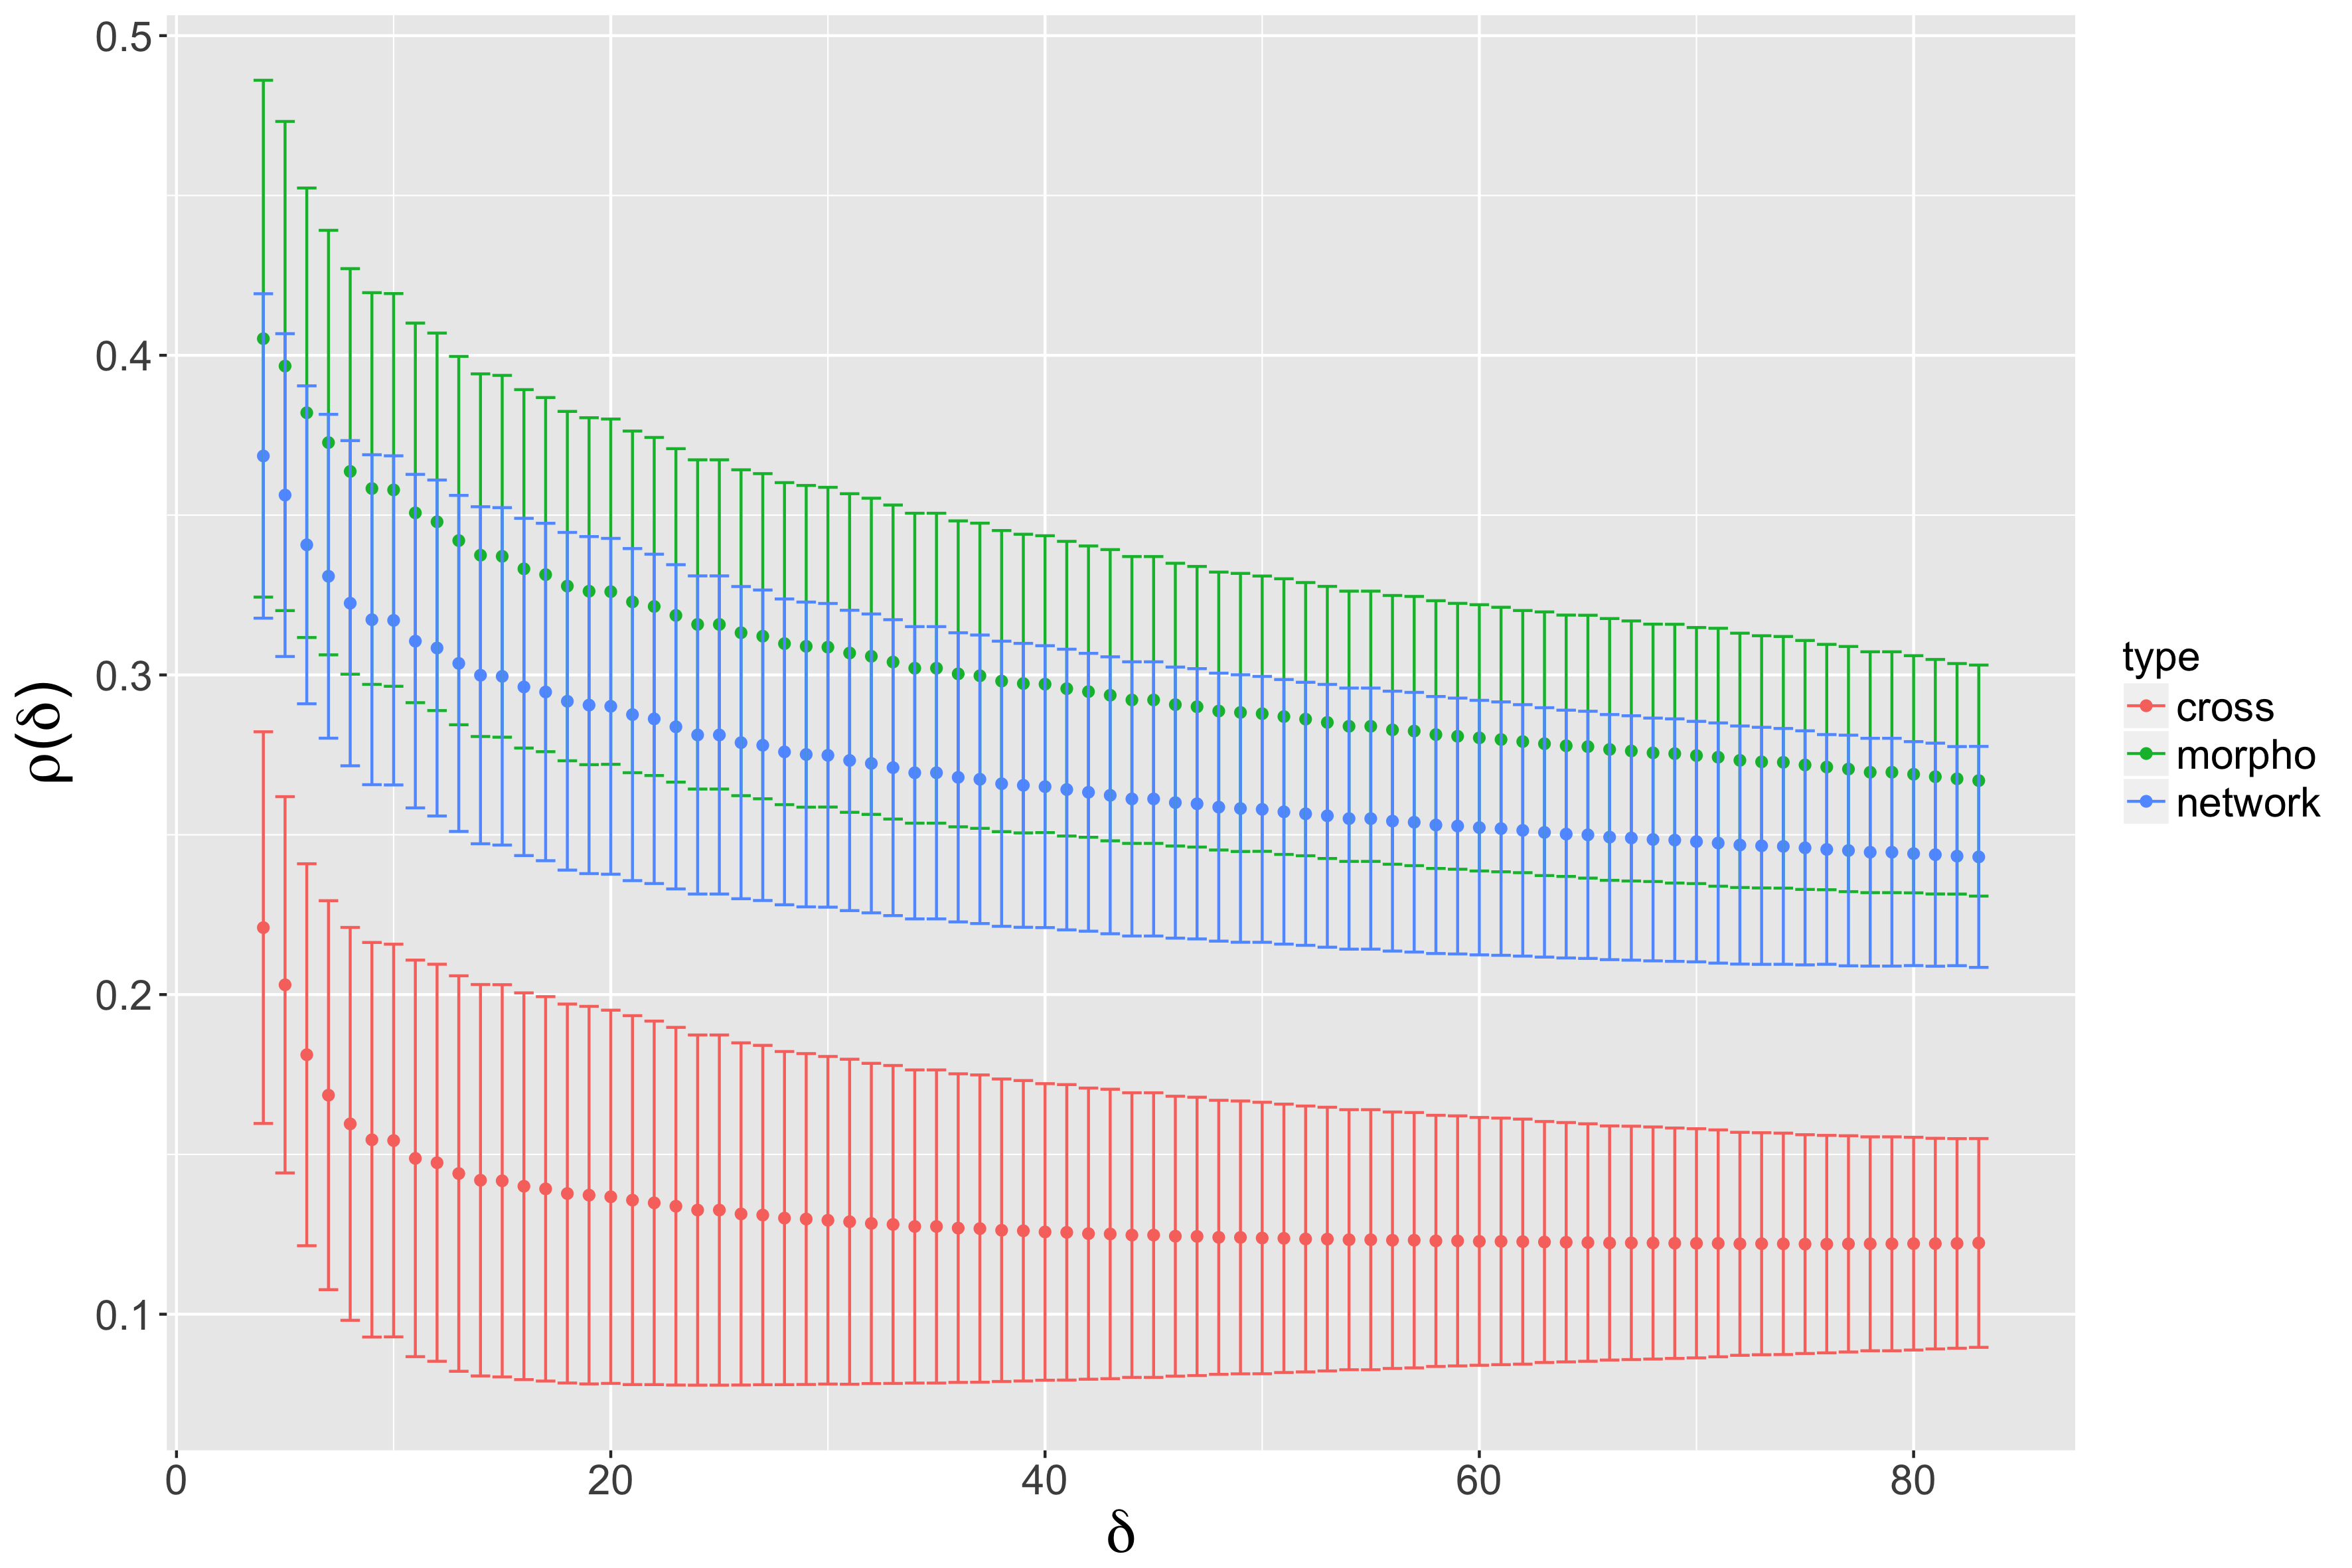
\includegraphics[width=0.48\linewidth]{Figures/StaticCorrelations/corrs-summary-meanabs_varyingdelta_bytype}\\
%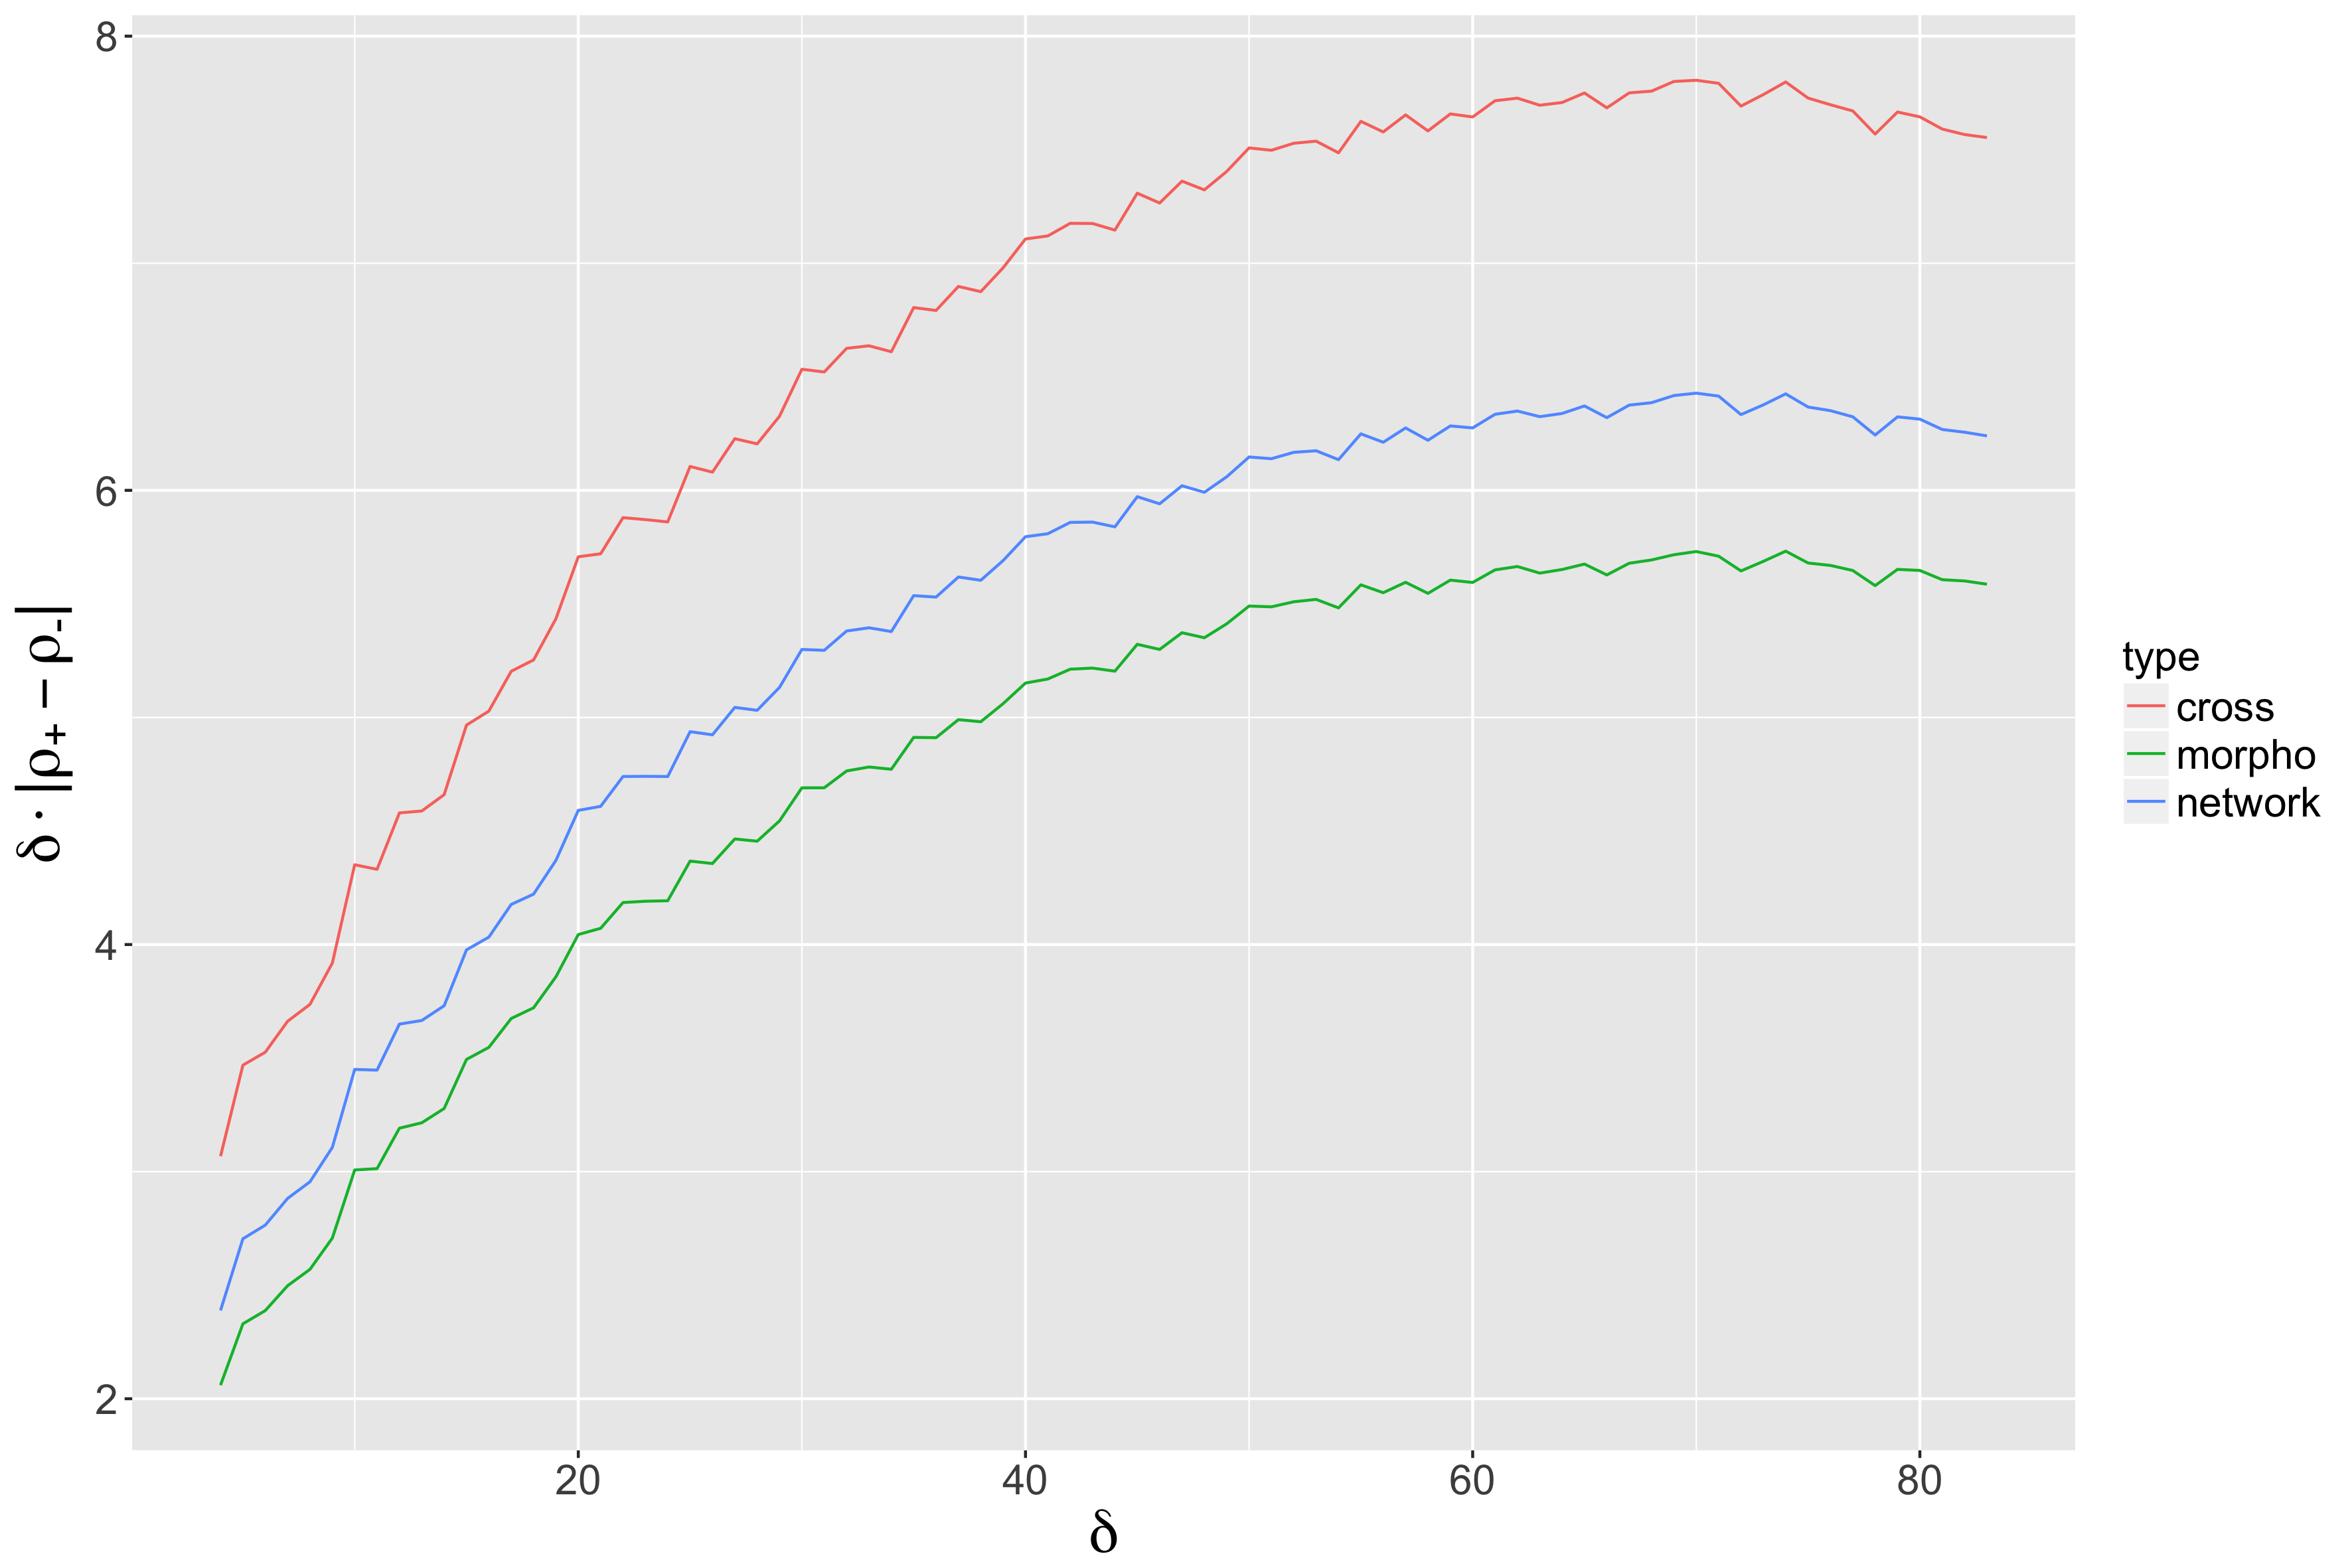
\includegraphics[width=0.48\linewidth]{Figures/StaticCorrelations/normalized_CI_delta}
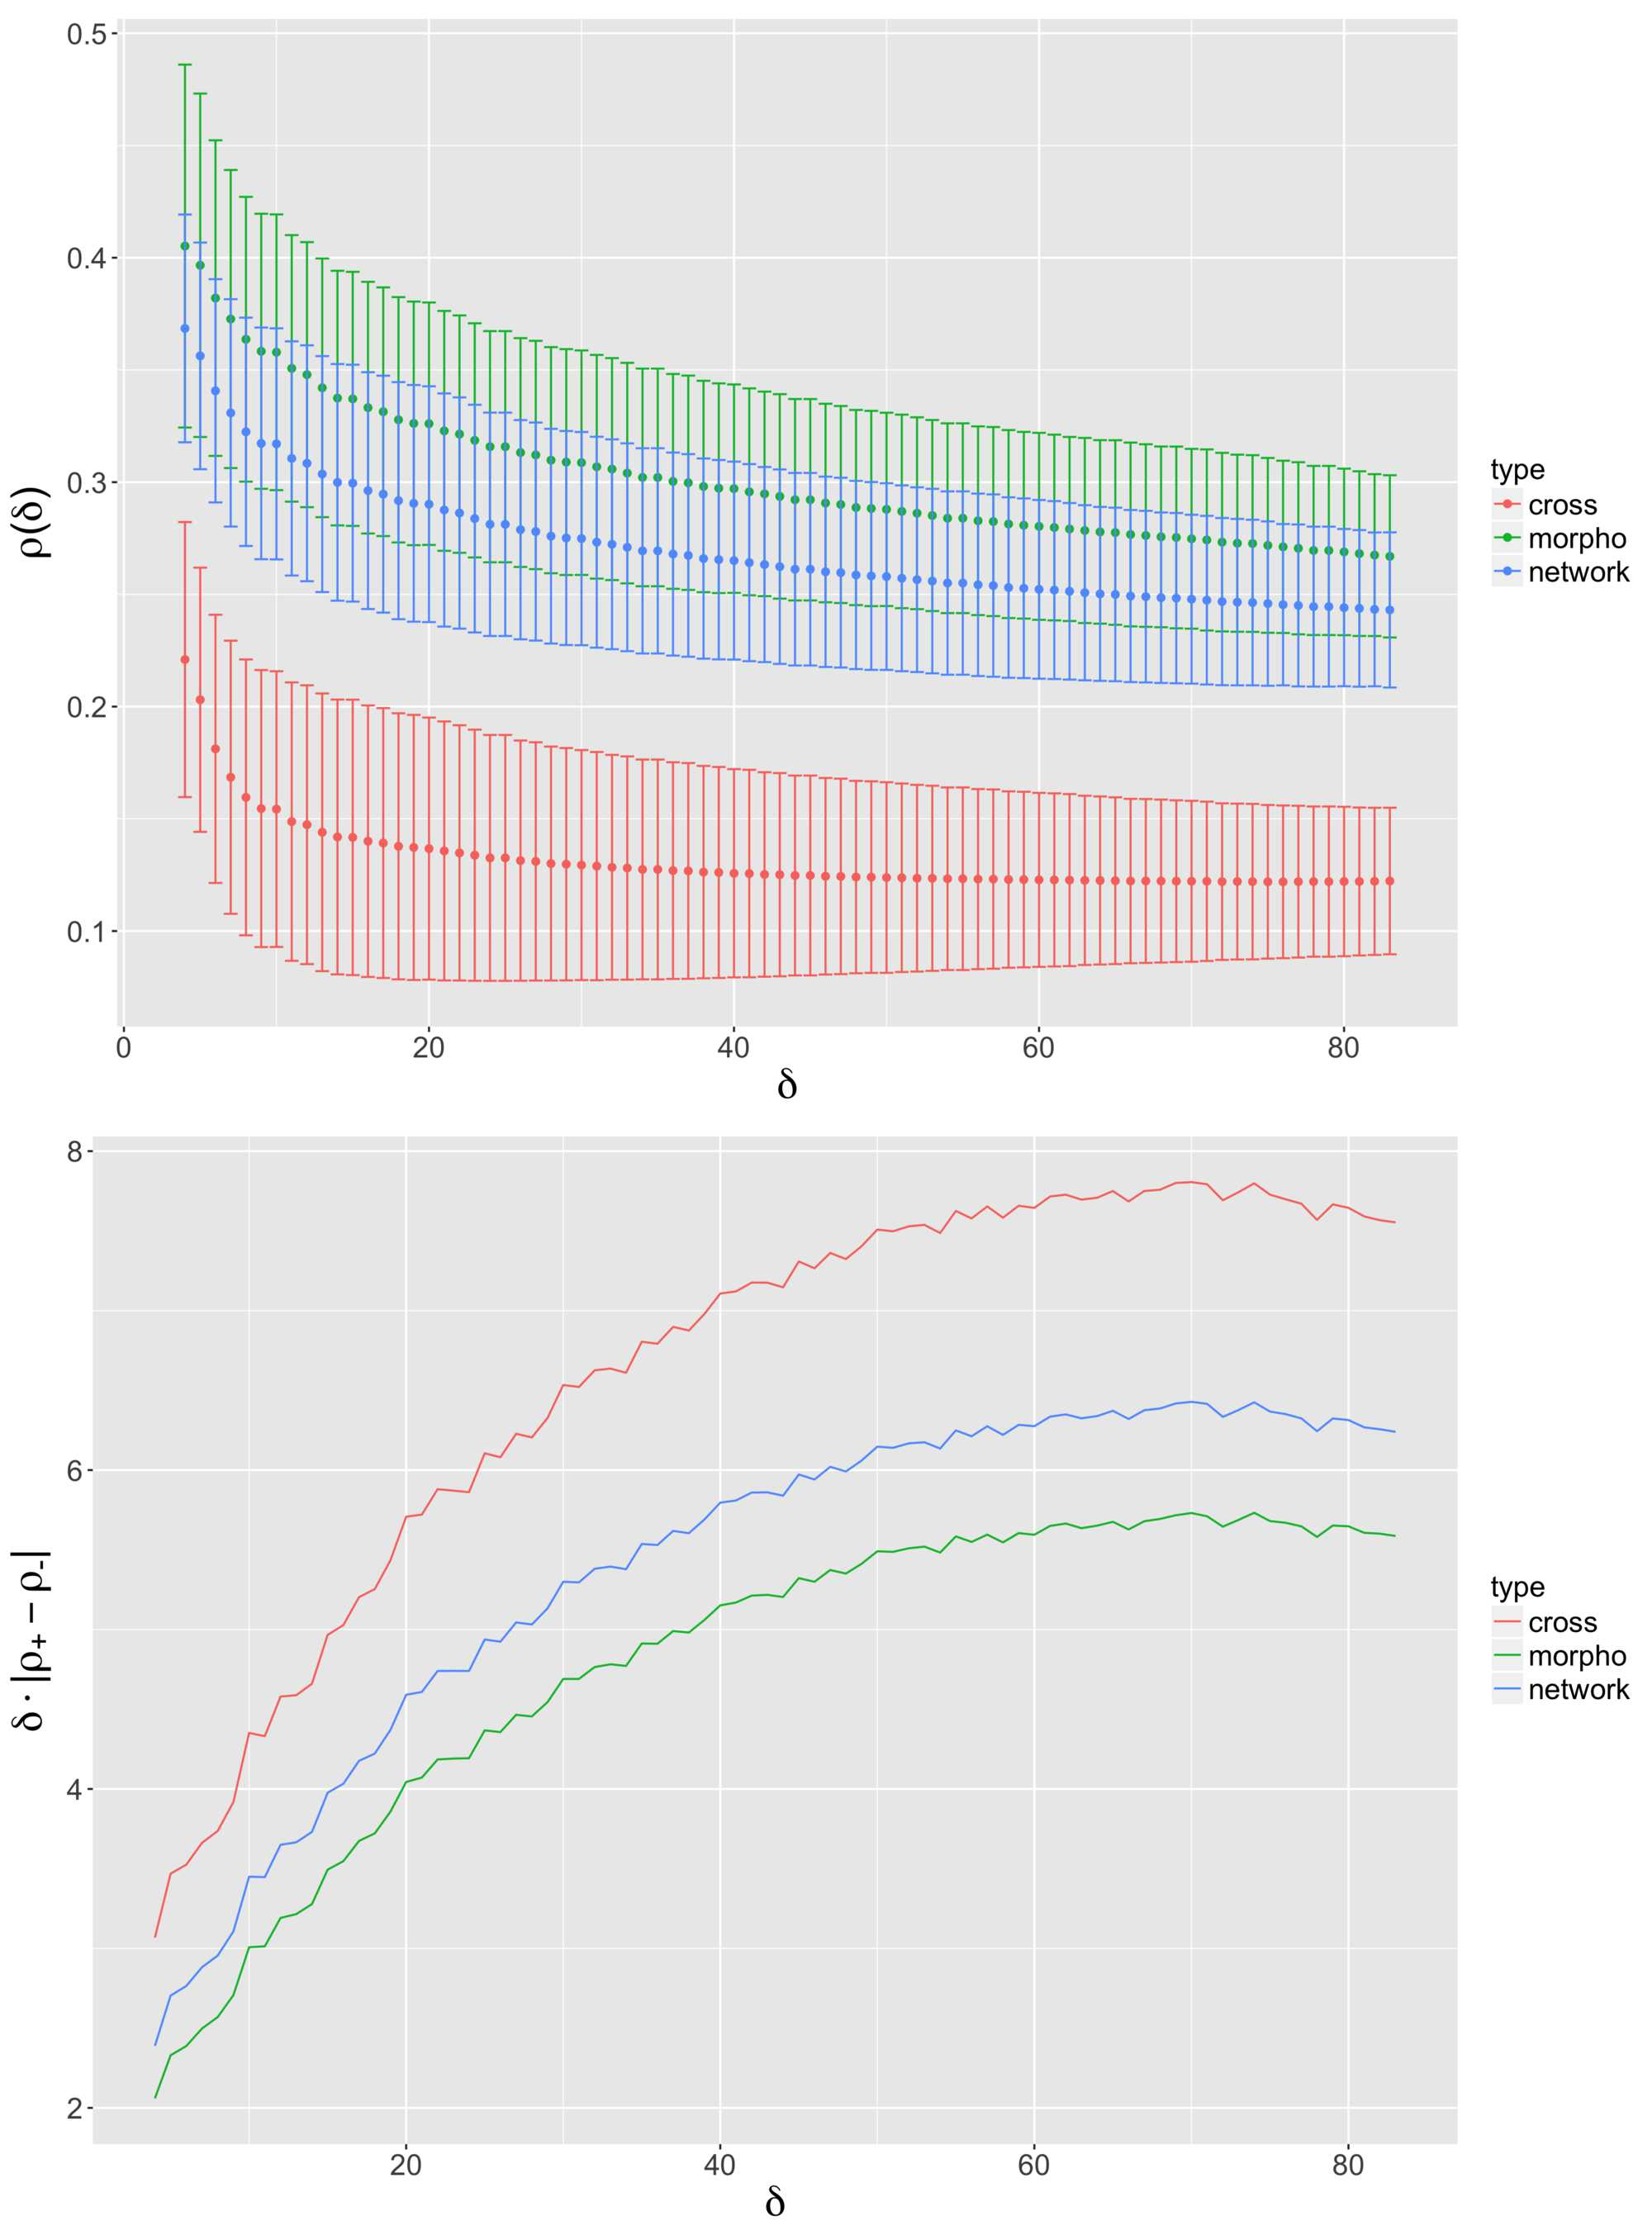
\includegraphics[width=\linewidth,height=0.85\textheight]{Figures/Final/4-1-3-fig-staticcorrs-corrsdistrib}
\caption[Variation of correlations with scale][Variation des corrélations avec l'échelle]{\textbf{Variation of correlations with scale.}\label{fig:staticcorrs:corrsdistrib}}{\textbf{Variation des corrélations avec l'échelle, pour les corrélations calculées sur l'Europe.} \textit{(Haut)} Correlations absolues moyennes et leur déviation standard, pour les différents blocs, en fonction de $\delta$ ; \textit{(Bas)} Taille de l'intervalle de confiance normalisée $\delta\cdot \left|\rho_{+} - \rho_{-}\right|$ (intervalle de confiance $\left[\rho_{-} , \rho_{+}\right]$ estimé par méthode de Fisher) en fonction de $\delta$ \label{fig:staticcorrs:corrsdistrib}}
\end{figure}
%%%%%%%%%%%%%%%%%%%%%%%%



%%%%%%%%%%%%%%%%%%
\subsubsection{Optimal Scales}{Echelles typiques}


\bpar{
We also compute the optimal bandwidth for a GWR PCA~\cite{harris2011geographically}. We beware to sample data accordingly to avoid local colinearity :\cite{wheeler2007diagnostic} colinearity in GWR
}{
Nous proposons d'autre part d'explorer la propriété éventuelle de multi-scalarité par extraction d'échelles endogène présentes dans les données. Une Analyse en Composantes Principales Géographique Pondérée (GWRPCA)~\cite{harris2011geographically} exploratoire suggère des poids et importances variables dans l'espace, ce qui est cohérent avec la non-stationnarité des structures de corrélation obtenue ci-dessus. Il n'y a a priori pas de raison pour que les échelles de variation des différents indicateurs soient strictement identiques. Nous proposons donc d'extraire les échelles typiques pour les relations croisées entre forme urbaine et forme de réseau.
}


\bpar{}{
Nous implémentons pour cela la méthode suivante : nous considérons un échantillon typique d'indicateurs (quatre pour chaque aspect, voir la liste en Table~\ref{tab:staticcorrelations:gwr}), et pour chaque indicateur nous formulons l'ensemble des modèles linéaires possibles en fonction des indicateurs opposés (réseau pour un indicateur morphologique, morphologique pour un indicateur de réseau), visant à capturer directement l'interaction sans contrôle sur le type de forme ou de réseau. Ces modèles sont alors ajustés par une Régression Géographique Pondérée (GWR) à portée optimale déterminée par critère d'information corrigé (AICc)\footnote{En utilisant le package R GWModel~\cite{gollini2013gwmodel}.}. Pour chaque indicateur, on retient le modèle ayant la meilleure valeur du critère d'information. Nous ajustons les modèles sur les données de la France, avec un noyau \emph{bisquare} et une portée adaptable en nombre de voisins.
}

\bpar{}{
Les résultats sont présentés en Table~\ref{tab:staticcorrelations:gwr}. Il est intéressant de noter dans un premier temps que l'ensemble des modèles ne comprend qu'une seule variable, suggérant des correspondances relativement directes entre topologie et morphologie. L'ensemble des indicateurs morphologiques est expliqué par la performance du réseau, c'est à dire la quantité de détour qu'il comprend. Au contraire, la topologie est expliquée par le Moran pour les centralités, et par l'entropie pour la performance et le nombre de sommets. On a ainsi une dissymétrie des relations, le réseau étant conditionné de manière plus complexe à la morphologie que la morphologie au réseau. Les ajustements sont bons ($R^2 > 0.5$) pour une majorité d'indicateurs, et les \emph{p-values} obtenues pour l'ensemble des modèles (constante et coefficient) sont inférieures à $10^-3$. Les échelles correspondant au modèle optimal sont quant à elles très localisées, de l'ordre de la dizaine de kilomètres, c'est à dire une plus grande variation que celle obtenue par les corrélations. Cette analyse confirme ainsi statistiquement d'une part la non-stationnarité, et d'autre part donne un point de vue complémentaire sur la question des échelles endogènes.
}

%bestmodels
%            indic             bestmodel      dist    bw        R2
%           <fctr>                <fctr>     <dbl> <dbl>     <dbl>
%1        distance  distance~networkPerf 11.609078    30 0.3145114
%2         entropy   entropy~networkPerf  8.795393    16 0.7511295
%3 meanBetweenness meanBetweenness~moran 12.294076    34 0.5776019
%4   meanCloseness   meanCloseness~moran 13.883025    44 0.2565047
%5           moran     moran~networkPerf  8.795393    16 0.4886164
%6     networkPerf   networkPerf~entropy  8.595512    15 0.8640510
%7           slope     slope~networkPerf  8.795393    16 0.6840567
%8          vcount        vcount~entropy  8.595512    15 0.8825783


%%%%%%%%%%%%%%%%%%
\begin{table}
\caption[Interrelations between network indicators and morphological indicators][Relation croisées entre indicateurs de réseau et morphologiques]{\textbf{Interrelations between network indicators and morphological indicators.}\label{tab:staticcorrelations:gwr}}{\textbf{Relation croisées entre indicateurs de réseau et morphologiques.} Chaque relation est ajustée par une Regression Géographique Pondérée, pour la portée optimale ajustée par AICc.\label{tab:staticcorrelations:gwr}}
\begin{tabular}{|l|l|l|l|}
\hline
Indicateur & Modèle & Portée (km) & Ajustement ($R^2$) \\ \hline
Distance moyenne $\bar{d}$ & $\bar{d} \sim v_0$ & 11.6 & 0.31 \\
Entropie $\mathcal{E}$  & $\mathcal{E} \sim v_0$ &  8.8  &0.75 \\
Moran $I$ & $I \sim v_0$ & 8.8 & 0.49 \\
Hiérarchie $\gamma$ & $\gamma \sim v_0$ & 8.8  & 0.68 \\\hline
\emph{Betwenness} moyenne $\bar{bw}$ & $\bar{bw} \sim I$ & 12.3 & 0.58 \\
\emph{Closeness} moyenne $\bar{cl}$ & $\bar{cl}\sim I$ & 13.9 & 0.26 \\
Performance $v_0$ & $v_0 \sim \mathcal{E}$ & 8.6  & 0.86 \\
Nombre de noeuds $\left|V\right|$ & $\left|V\right| \sim \mathcal{E}$ & 8.6  & 0.88 \\\hline
\end{tabular}
\end{table}
%%%%%%%%%%%%%%%%%%



%%%%%%%%%%%%%%%%%%
%\subsubsection{Spatial non-stationarity and non-ergodicity}{Non-stationnarité spatiale et non-ergodicité}



%%%%
%% -- ON HOLD : not useful for further demo --

%\paragraph{Formalization}{Formalisation}
%\bpar{
%We propose to formalize our empirical findings. Let $Y_i\left[\vec{x},t\right]$ a spatio-temporal stochastic process. We showed following assumptions:
%\begin{enumerate}
%\item Local spatial autocorrelation is present and bounded by $l_{\rho}$ (in other words the processes are continuous in space) : at any $\vec{x}$ and $t$, $\left|\rho_{\norm{\Delta \vec{x}} < l_{\rho}}\left[Y_i (\vec{x}+\Delta \vec{x},t), Y_i (\vec{x},t) \right]\right| > 0$.
%\medskip
%\item Processes are locally parametrized : $Y_i = Y_i\left[\alpha_i\right]$, where $\alpha_i (\vec{x})$ varies with $l_{\alpha}$, with $l_{\alpha} \gg l_{\rho}$ and weakly locally stationary in space.
%\medskip
%%\item Spatial correlations between processes have a sense at an intermediate scale $l$ such that $l_{\alpha}\gg l \gg l_{\rho}$.
%%\item Processes covariance stationarity times scale as $\sqrt{l}$.
%%\item Local ergodicity is present at scale $l$ and dynamics are locally chaotic.
%\item Processes are multi-scalar : since $\rho(\delta = \infty) > \rho (\delta = 0 )$, a necessary non-linear correction on processes spatial averages in correlation computation is present.
%% add computation in supplementary materials / papers. -> later
%\end{enumerate}
%}{
%Formalisons les conclusions empiriques obtenues. Soit $Y_i\left[\vec{x},t\right]$\comment[FL]{?} un processus stochastique\comment[FL]{faut-il que ce soit generique ? le dire alors} spatio-temporel. Nous avons alors les hypothèses suivantes :
%\begin{enumerate}
%\item L'autocorrelation spatiale locale existe en dessous d'une échelle minimale $l_0$ (en d'autres termes le processus est continu dans l'espace) : pour tout $\vec{x}$ et $t$, on a $\left|\rho_{\norm{\Delta \vec{x}} < l_0}\left[Y_i (\vec{x}+\Delta \vec{x},t), Y_i (\vec{x},t) \right]\right| \neq 0$.
%\item Les processus sont localement paramétrés\comment[FL]{?} : $Y_i = Y_i\left[\alpha_i\right]$, où $\alpha_i (\vec{x})$ varie à l'échelle $l_{\alpha}$, avec $l_{\alpha} \gg l_0$, c'est à dire qu'il est localement stationnaire dans l'espace.
%\item Les processus sont multi-scalaires\comment[FL]{def}[sens ci dessus : superposition processus a differentes echelles] : comme $\rho(\delta = \infty) > \rho (\delta = 0 )$\comment[FL]{aucun sens}, une nécessaire correction non-linéaire sur les moyennes spatiales des processus est présente dans le calcul des corrélations.\comment[FL]{c'est hyperflou et donc non-reproductible}[cf demo en annexe]
%\end{enumerate}
%}



%\bpar{
%}{
%Nous proposons de suggérer un lien entre les propriétés de non-stationnarité et la non-ergodicité des systèmes. Nous rappelons qu'il s'agit d'un aspect essentiel postulé par la Théorie Evolutive~\cite{pumain2012urban}, conduisant à discuter les interprétation universelles des systèmes urbains proposées par les théories du Scaling~\cite{bettencourt2007growth}.
%}

%\bpar{}{
%Précisons d'abord ce que nous entendons par propriétés d'ergodicité dans notre cas. Nous distinguerons ergodicité \emph{locale}, c'est à dire ergodicité dans un voisinage spatial des points considérés, et ergodicité \emph{globale}, c'est à dire vérifiée sur l'ensemble de définition spatial du processus. Par ailleurs, nous séparerons espace et temps (nos données étant statiques) et considérerons ergodicité \emph{spatiale} (moyenne d'ensemble correspondant à la moyenne spatiale, typiquement utilisée en géosciences~\cite{davis1994wavelet}) et ergodicité \emph{temporelle} (moyenne d'ensemble correspondant à la moyenne temporelle, utilisée en analyse de séries temporelles~\cite{kantz2004nonlinear}). Nous nous intéresserons plus particulièrement à l'ergodicité spatiale locale et globale.
%}

%\bpar{}{
%Notons que nous avons déjà implicitement supposé ergodicité spatiale locale (pour les processus $X_i\cdot X_{i'}$ si les $X_i$ sont les indicateurs), lorsque nous avons estimé les corrélations sur des fenêtres spatiales. Cette hypothèse parait raisonnable, au sens où un régime local se manifestera de manière aléatoire sur ses différentes instances locales dans le cas d'indicateurs effectivement stochastiques à cette échelle (on pourra considérer les résultats de simulation de~\ref{sec:densitygeneration} pour se donner une idée). Empiriquement, l'existence d'entités cohérentes pour les valeurs des corrélations dans l'espace suggère qu'on peut se placer dans un cas analogue.
%}

%\cite{crutchfield1987phenomenology}




%%%%%%%%%%%%%%%%%%
\subsubsection{Developments}{Développements}



\bpar{
We show the regional nature of network-territories interactions, in particular the non-ergodicity of urban systems on \textbf{the interaction these components}. No direct results on time dynamics, but indirect : spatio-temporal processes do not have same speed and react/diffuse differently.
}{
Nous avons montré ainsi montré empiriquement la non-stationnarité des interactions entre morphologie de la distribution des population et topologie du réseau routier. Divers développements de cette analyse sont possibles.
}

% la non-ergodicité du système territorial concernant l'interaction entre ces composantes.\comment[FL]{et alors ? par ailleurs vu que tu n'as jamais vraiment parlé de villes, tu ne peux pas avoir montré ce que tu prétends avoir montré} Nous n'extrayons pas de résultats directs sur les dynamiques par ces analyses statiques, mais pouvons postuler des résultats indirects :




%\paragraph{Universality}{Universalité}
\bpar{
In \cite{10.1371/journal.pone.0107042} density grids for other countries across the world are provided\footnote{available at \url{http://www.worldpop.org.uk/}}. The analysis may be repeated to other regions of the world, to compare the correlation regimes and test if urban system properties stay the same. We can expect different regimes for the United States compared to Europe for example, but the discrepancy needs still to be investigated~\cite{bretagnolle2010comparer}.
}{
Des grilles de densité de population existent pour l'ensemble des régions du monde, comme par exemple celles fournies par~\cite{10.1371/journal.pone.0107042}\footnote{Disponibles à \url{http://www.worldpop.org.uk/}. La variabilité potentielle de la qualité des données selon les zones doit toutefois amener une prudence dans leur utilisation.}. L'analyse peut être répétée pour d'autres régions, pour comparer les régimes de corrélations et tester si les propriétés des systèmes urbains restent les mêmes, en gardant à l'esprit les difficultés liées aux différences de qualité dans les données.
}

% On peut s'attendre à des régimes très différents pour les Etats-Unis en comparaison à l'Europe par exemple~\cite{bretagnolle2010comparer}, mais la différence se devrait d'être étudiée quantitativement, pour par exemple dégager des caractéristiques différentes d'interactions entre réseaux et territoires.



\bpar{
Still points to explore :
\begin{itemize}
\item variable correlations areas (size and shape in space)
\item same work on cities population/train network data, which are also dynamical databases : extrapolation of ergodicity parameters ?
\item correlations of returns : link between $\rho\left[\Delta_t Y\right]$ and $\rho\left[\Delta_x Y\right]$ (more difficult : if pure local ergodicity, $\exists$ a permutation making the correspondance) % may be difficult to identify 
\item Link between $\Delta_{\delta}\rho (\delta)$ and process derivatives ?
\end{itemize}
}{
La recherche d'échelles locales, c'est à dire avec une fenêtre d'estimation adaptative en taille et forme pour les corrélations, permettrait de mieux comprendre la façon dont les processus influent localement sur leur voisinage. Le critère de validation de la taille de la fenêtre resterait à déterminer : il peut s'agir comme ci-dessus de portée optimale pour des modèles explicatifs ajustés localement.
}

\bpar{}{
La question de l'ergodicité devrait également être explorée sur des bases dynamiques, en comparant les échelles de temps et d'espace d'évolution des processus, ou plus précisément les corrélations entre les variations dans le temps et celles dans l'espace, mais la question de l'existence de bases de données assez fines dans le temps paraît problématique. L'étude d'un lien entre la dérivée de la corrélation en fonction de la taille de la fenêtre et les dérivées des processus est également une piste pour obtenir des informations indirectes sur la dynamique à partir des données statiques.
}

% \comment[FL]{je suis d'accord cela se rapproche un peu de la demarche d'indicateur d'acentrisme}

\bpar{}{
Enfin, la recherche de classes de processus sur lesquels il est possible d'établir directement la relation entre corrélations spatiales et corrélations temporelles, est une direction possible de recherche. Celle-ci est hors de portée de ce présent travail, mais ouvrirait des perspectives pertinentes sur la co-évolution, puisque celle-ci implique évolution dans le temps et en isolation dans l'espace, et donc une relation complexe entre covariances spatiales et temporelles. 
}

% On suggère par exemple en Appendice~\ref{sec:spatiotempcorrs} des cas idéaux pour lesquels un lien peut être directement obtenu, comme le cas de processus territoriaux ayant une caractérisation ondulatoire par exemple.



%%%
% ouverture covariance spatio-temporelle:
% \cite{wikle1999dimension} space time Kalman filter
% \cite{crutchfield1987phenomenology} spatio-temporal chaos
% \cite{fuentes2006testing} separability of space-time covariance functions
% \cite{rand1995using} : application of spatio-temporal chaos to CA model of an ecosystem
% \cite{aubry1991spatiotemporal} orthogonal decomposition in space and time
% https://projecteuclid.org/download/pdf_1/euclid.aop/1176996986 other def of ergodicity (convergence of proba matrix) : ?







\stars




Cette section nous a donc permis d'étudier les propriétés de non-stationnarité des caractéristiques morphologiques des territoires et des réseaux, et de leur interactions en termes de corrélations statiques. Les indicateurs calculés seront également utiles par la suite.


Nous proposons dans la section suivante de nous attaquer à une approche statistique de la co-évolution, correspondant à la définition intermédiaire que nous en avons donné. Contrairement à l'approche précédente, celle-ci sera basée sur les dynamiques.


\stars



